% !TEX root = ../../../main.tex

\toggletrue{image}
\toggletrue{imagehover}
\chapterimage{1337_part_2}
\chapterimagehover{Trivia: Elaine is actually her middle name.}
\chapterimagetitle{\uppercase{1337: Part 2}}
\chapterimageurl{https://xkcd.com/342/}

\chapter{Routenplaner}
\label{chapter-routenplaner}

Die primäre Funktion von Google Maps (\url{https://www.google.de/maps}) ist das Planen von Routen. \autoref{figure-google-maps} zeigt eine Routenplanung von der Kantonsschule Wettingen zur Kantonsschule Baden mit dem Fahrrad.

\begin{figure}[htb]
	\centering
	\includegraphics[scale=0.25]{google_maps_kswe_ksb}
	\caption{Es gibt mindestens 2 Routen zur Kantonsschule Baden. Eine Route ist etwas kürzer.}
	\label{figure-google-maps}
\end{figure}

Die typische Fragestellung bei einer Routenplanung lautet also: \textbf{Wie komme ich am kürzesten/schnellsten/günstigsten von A nach B?} Wir werden in diesem Kapitel einen Algorithmus kennenlernen, der die kürzeste Route zwischen zwei Orten ermitteln kann. Die Lernziele für dieses Kapitel lauten:

\newcommand{\routenplanerLernziele}{
\protect\begin{todolist}
\item Sie erklären die Methode der Abstraktion und Gleichformung.
\item Sie modellieren eine Strassenkarte durch einen gewichteten Graphen.
\item Sie erklären, was wir in einem gewichteten Graphen unter einem kürzesten Weg verstehen.
\item Sie erklären, was ein Brute-Force-Algorithmus ist und warum wir diesen für die Routenplanung nicht einsetzen können.
\item Sie wenden den Algorithmus von Dijkstra an.
\end{todolist}
}

\lernziel{\autoref{chapter-routenplaner}, \nameref{chapter-routenplaner}}{\protect\routenplanerLernziele}

\routenplanerLernziele

\section{Modellierung einer Strassenkarte}

Betrachten wir die fiktive Strassenkarte aus \autoref{figure-strassenkarte-1}. Wir möchten den \textbf{kürzesten Weg} von \textbf{Imstadt} nach \textbf{Oppenheim} finden. Wenn wir verschiedene Weg ausprobieren, können wir zur korrekten Lösung kommen. In diesem Fall ist es der Weg von Imstadt nach Pappstadt und dann nach Krupsing. Von Krupsing weiter über Fluxing nach Oppenheim. Dies sind insgesamt $24,6$ km.

\begin{figure}[htb]
\centering
\includegraphics[scale=0.425]{strassenkarte_abenteuer_informatik}
\caption{Strassenkarte mit teilweise fiktiven Orten \cite{abenteuer-informatik}. Alle Streckenangaben in Kilometer.}
\label{figure-strassenkarte-1}
\end{figure}

Wir werden nun in mehreren Schritten die Strassenkarte so \say{umbauen}, dass wir eine Darstellung erhalten, die ein Computerprogramm verarbeiten kann.	

\subsection{Methode der Abstraktion}

Wir wandeln die Strassenkarte in ein Format um, welches wir einfach in ein Computerprogramm übersetzen können. Wir verwenden dabei zunächst die folgende Herangehensweise.

\begin{definition}[Methode der Abstraktion]
In der zur Verfügung stehenden Information stecken oft sowohl relevante als auch unwesentliche Anteile. Durch \textbf{Abstraktion} reduzieren wir die Information auf die wesentlichen Aspekte bezüglich der \textbf{aktuellen} Problemlösung.
\end{definition}

Bei der Routenplanung steht die Strassenkarte als Information zur Verfügung. Wir möchten nun den \textbf{kürzesten Weg von A nach B} ermitteln. Welche Informationen sind bei einer Strassenkarte dafür das Wesentliche? Wir sind mit einem \say{idealen} Auto/eBike/eScooter unterwegs und halten uns immer strikt an alle Vorgaben. \autoref{table-routenplanung-abstraktion} zeigt die zentralen Informationen der Strassenkarte mit einer jeweiligen Begründung, ob die Information relevant ist oder nicht.

\begin{table}[htb]
\centering
\begin{tabular}{|p{3.5cm}|p{10cm}|}
\hline
\textbf{Information} & \textbf{Wesentlich?} \\ \hline
Namen der Städte & \textbf{Ja!} Wenn wir nicht wissen, welche Stadt wie heisst, kann auch nicht der kürzeste Weg zwischen zwei Städten bestimmt werden. \\ \hline
Position der Städte & \textbf{Nein!} Es ist uns egal, wo sich die Städte genau befinden. Relevant sind nur die Strassen zwischen den Städten. \\ \hline
Grösse der Städte & \textbf{Nein!} Dies spielt für die Routenplanung keine Rolle. Auch die farblichen Markierungen der Kreise sind irrelevant. \\ \hline
Verlauf der Strassen & \textbf{Nein!} Es kommt nur auf die Strecke an, nicht auf den Verlauf. \\ \hline
Länge der Strassen & \textbf{Ja!} Um die Reisestrecke zu summieren, benötigen wir die einzelnen Strecken zwischen den Orten. \\ \hline
Namen und Nummern der Strassen & \textbf{Nein!} Zumindest zur Bestimmung der kürzesten Strecke irrelevant. \\ \hline
Strassentyp & \textbf{Nein!} Da es nur auf die Entfernungen, nicht auf Zeit ankommt, ist egal, ob Autobahn oder Feldweg gefahren wird.\\ \hline
Strasse führt von ... nach ... & \textbf{Ja!} Wir benötigen die Information, von welcher Stadt zu welcher anderen eine Strasse führt. \\ \hline
Landschaftliche Information & \textbf{Nein!} Ist zwar nett bei einer Autofahrt, aber völlig irrelevant. \\ \hline
\end{tabular}
\caption{Nur drei dieser zehn Punkte sind wirklich wichtig für die Routenplanung.}
\label{table-routenplanung-abstraktion}
\end{table}

Wenn wir konsequent alles Unnötige von der Strassenkarte entfernen und nur diejenigen Elemente beibehalten, welche wirklich massgeblich sind, dann können wir die Strassenkarte neu zeichnen und erhalten die Darstellung in \autoref{figure-graph-strassekarte-1}. Wenn wir die Darstellung aus \autoref{figure-graph-strassekarte-1} genauer betrachten, dann können wir erkennen, dass es noch ein paar Besonderheiten gibt:

\begin{itemize}
\item Städte und Strassenkreuzungen werden konzeptuell noch unterschieden (Städte besitzen eine Bezeichnung, Kreuzungen nicht).
\item Es gibt noch zwei direkte Strassen von Imstadt nach Pappstadt. Welche sollen wir nehmen?
\item Es gibt noch eine \say{Schleife} bei Delgar. Ist dies sinnvoll?
\end{itemize}

Wir gehen diese Gesichtspunkte im nächsten Abschnitt an.

\begin{figure}
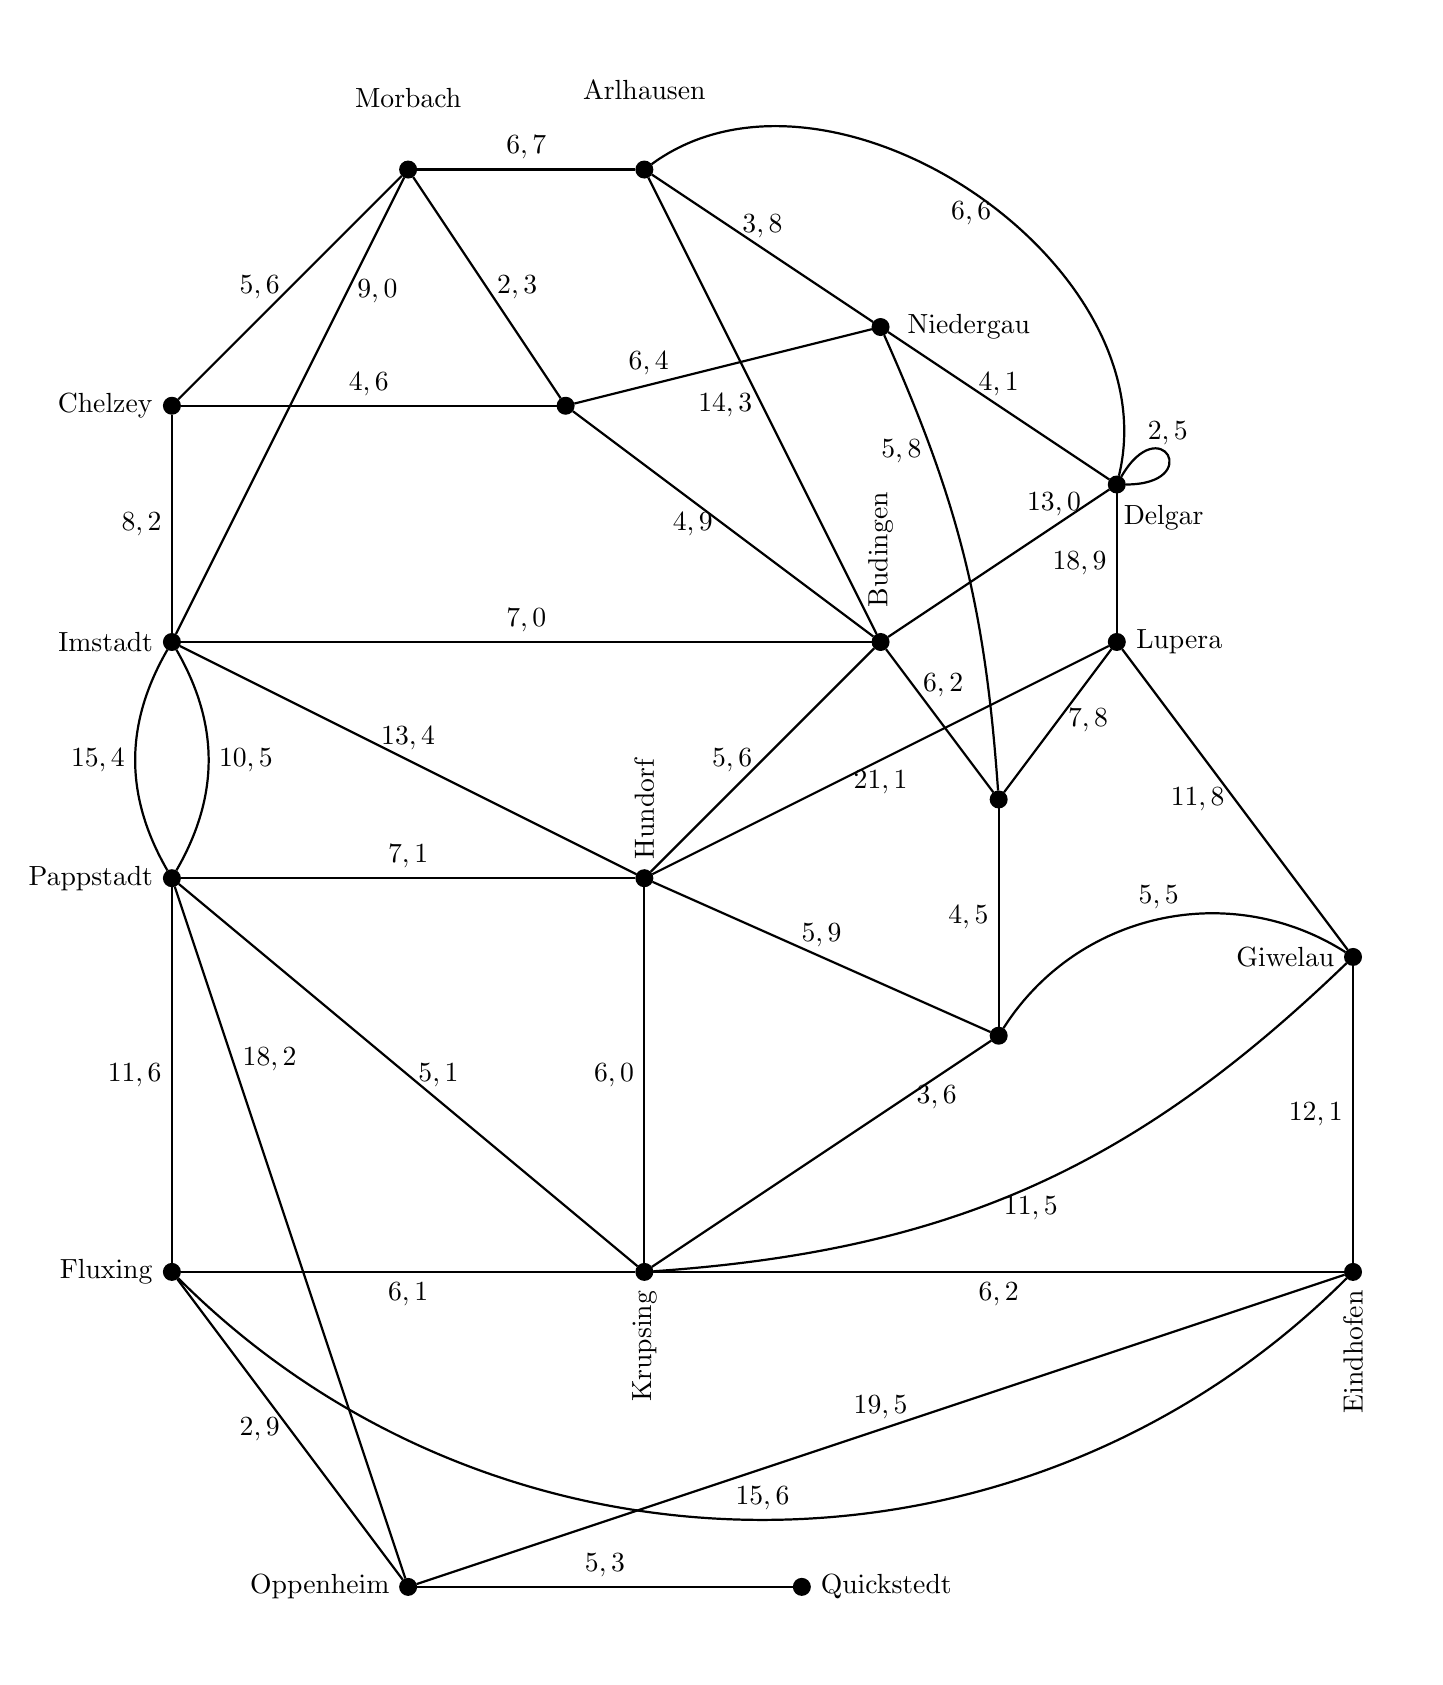
\begin{tikzpicture}
\begin{scope}[every node/.style={circle, thick, fill, draw, inner sep=0cm, minimum size=0.2cm}]
    \node[label={[label distance=0.1cm]180:Imstadt}] (v1) at (-3,0) {};
    \node[label={[label distance=0.1cm]180:Chelzey}] (v2) at (-3,3) {};
    \node[label={[label distance=0.1cm]90:Morbach}] (v3) at (0,6) {};
    \node (v4) at (2,3) {};
    \node[label={[label distance=0.3cm]90:\rotatebox{90}{Budingen}}] (v5) at (6,0) {};
    \node[label={[label distance=0.1cm]90:\rotatebox{90}{Hundorf}}] (v6) at (3,-3) {};
    \node[label={[label distance=0.1cm]180:Pappstadt}] (v7) at (-3,-3) {};
    \node[label={[label distance=0.1cm]90:Arlhausen}] (v8) at (3,6) {};
    \node[label={[label distance=0.2cm]0:Niedergau}] (v9) at (6,4) {};
    \node[label={[label distance=0.1cm]350:Delgar}] (v10) at (9,2) {};
    \node (v11) at (7.5,-2) {};
    \node[label={[label distance=0.1cm]0:Lupera}] (v12) at (9,0) {};
    \node[label={[label distance=0.1cm]180:Giwelau}] (v13) at (12,-4) {};
    \node (v14) at (7.5,-5) {};
    \node[label={[label distance=0.1cm]270:\rotatebox{90}{Eindhofen}}] (v15) at (12,-8) {};
    \node[label={[label distance=0.1cm]270:\rotatebox{90}{Krupsing}}] (v16) at (3,-8) {};
    \node[label={[label distance=0.1cm]180:Fluxing}] (v17) at (-3,-8) {};
    \node[label={[label distance=0.1cm]180:Oppenheim}] (v18) at (0,-12) {};
    \node[label={[label distance=0.1cm]0:Quickstedt}] (v19) at (5,-12) {};
\end{scope}
\begin{scope}[every edge/.style={draw=black, thick}]
    \path (v1) edge node[left] {$8,2$} (v2);
    \path (v1) edge node[near end, right] {$9,0$} (v3);
    \path (v1) edge node[above] {$7,0$} (v5);
    \path (v1) edge node[above] {$13,4$} (v6);
    \path (v1) edge[bend left] node[right] {$10,5$} (v7);
    \path (v1) edge[bend right] node[left] {$15,4$} (v7);
    \path (v2) edge node[left] {$5,6$} (v3);
    \path (v2) edge node[above] {$4,6$} (v4);
    \path (v3) edge node[right] {$2,3$} (v4);
    \path (v3) edge node[above] {$6,7$} (v8);
    \path (v4) edge node[left] {$4,9$} (v5);
    \path (v4) edge node[near start, above] {$6,4$} (v9);
    \path (v5) edge node[left] {$5,6$} (v6);
    \path (v5) edge node[left] {$14,3$} (v8);
    \path (v5) edge node[near end, above] {$13,0$} (v10);
    \path (v5) edge node[near start, right] {$6,2$} (v11);
    \path (v6) edge node[above] {$7,1$} (v7);
    \path (v6) edge node[above] {$5,9$} (v14);
    \path (v6) edge node[left] {$6,0$} (v16);
    \path (v7) edge node[right] {$5,1$} (v16);
    \path (v7) edge node[left] {$11,6$} (v17);
    \path (v7) edge node[right, near start] {$18,2$} (v18);
    \path (v8) edge node[above] {$3,8$} (v9);
    \path (v8) edge[bend left=70, below] node {$6,6$} (v10);
    \path (v9) edge node[above] {$4,1$} (v10);
    \path (v9) edge[bend left=10] node[near start, left] {$5,8$} (v11);
    \path (v10) edge[loop, min distance=10mm, in=0, out=60, looseness=10] node[above] {$2,5$} (v10);
    \path (v10) edge node[left] {$18,9$} (v12);
    \path (v11) edge node[left] {$4,5$} (v14);
    \path (v12) edge node[right] {$7,8$} (v11);
    \path (v12) edge node[left] {$11,8$} (v13);
    \path (v12) edge node[below] {$21,1$} (v6);
    \path (v13) edge node[left] {$12,1$} (v15);
    \path (v13) edge[bend left=20, below] node {$11,5$} (v16);
    \path (v14) edge node[right, near start] {$3,6$} (v16);
    \path (v14) edge[bend left=45, above] node {$5,5$} (v13);
    \path (v15) edge node[below] {$6,2$} (v16);
    \path (v15) edge[bend left=45, above] node {$15,6$} (v17);
    \path (v15) edge node[above] {$19,5$} (v18);
    \path (v16) edge node[below] {$6,1$} (v17);
    \path (v17) edge node[left] {$2,9$} (v18);
    \path (v18) edge node[above] {$5,3$} (v19);
\end{scope}
\end{tikzpicture}
\caption{Die Strassenkarte nach der Methode der Abstraktion.}
\label{figure-graph-strassekarte-1}
\end{figure}

\clearpage

\subsection{Methode der Gleichformung}

Algorithmen können einfacher erstellt werden, wenn die Elemente der Problemstellung möglichst einheitlich sind. Wir möchten uns möglichst wenige Sonderfälle kümmern. Dies erreichen wir dadurch, in dem wir das Problem möglichst gleichförmig darstellen.

\begin{definition}[Methode der Gleichformung]
Wir versuchen, die verschiedenen Facetten eines Problems auf die \textbf{gleichen Grundelemente} zurückzuführen. Dadurch wird einerseits das Problem übersichtlicher und andererseits benötigen wir weniger Lösungsansätze: Für gleichförmige Teilprobleme kann der gleiche Lösungsansatz verwendet werden.
\end{definition}

Mit der Methode der Gleichformung können wir die Darstellung aus \autoref{figure-graph-strassekarte-1} weiter vereinfachen und einheitlicher darstellen.

\begin{itemize}
	\item \textbf{Strassenkreuzungen und Städte vereinheitlichen}: Aus einer abstrakten Perspektive sind für die Routenplanung Städte und Kreuzungen identisch: beide Orte ermöglichen einen Strassenwechsel. Wir behandeln Strassenkreuzungen also als fiktive Städte und geben den Kreuzungen die \say{Namen} $X$, $Y$ und $Z$.
	\item \textbf{Schleifen entfernen}: Eine Schleife, wie es bei Delgar vorkommt, ergibt für die Bestimmung des kürzesten Wegs keinen Sinn. Wenn wir nach Delgar wollen, dann würde die Schleife die Strecke nur vergrössern. Wir können somit Schleifen prinzipiell entfernen.
	\item \textbf{Doppelte Verbindungen entfernen}: Für die Bestimmung des kürzesten Wegs kommt von zwei möglichen Strecken zwischen zwei benachbarten Orten nur die kürzere Strecke infrage. Wenn wir die Auswahl haben zwischen der Strecke über $15,4$ km von Imstadt nach Pappstadt und der Strecke über $10,4$ km, dann entscheiden wir uns für die kürzere Strecke. Wir können somit bei zwei direkten Strecken zwischen zwei Orten die längere Strecke entfernen. 
\end{itemize}


\begin{figure}[htb]
\centering
\resizebox{!}{11cm}{
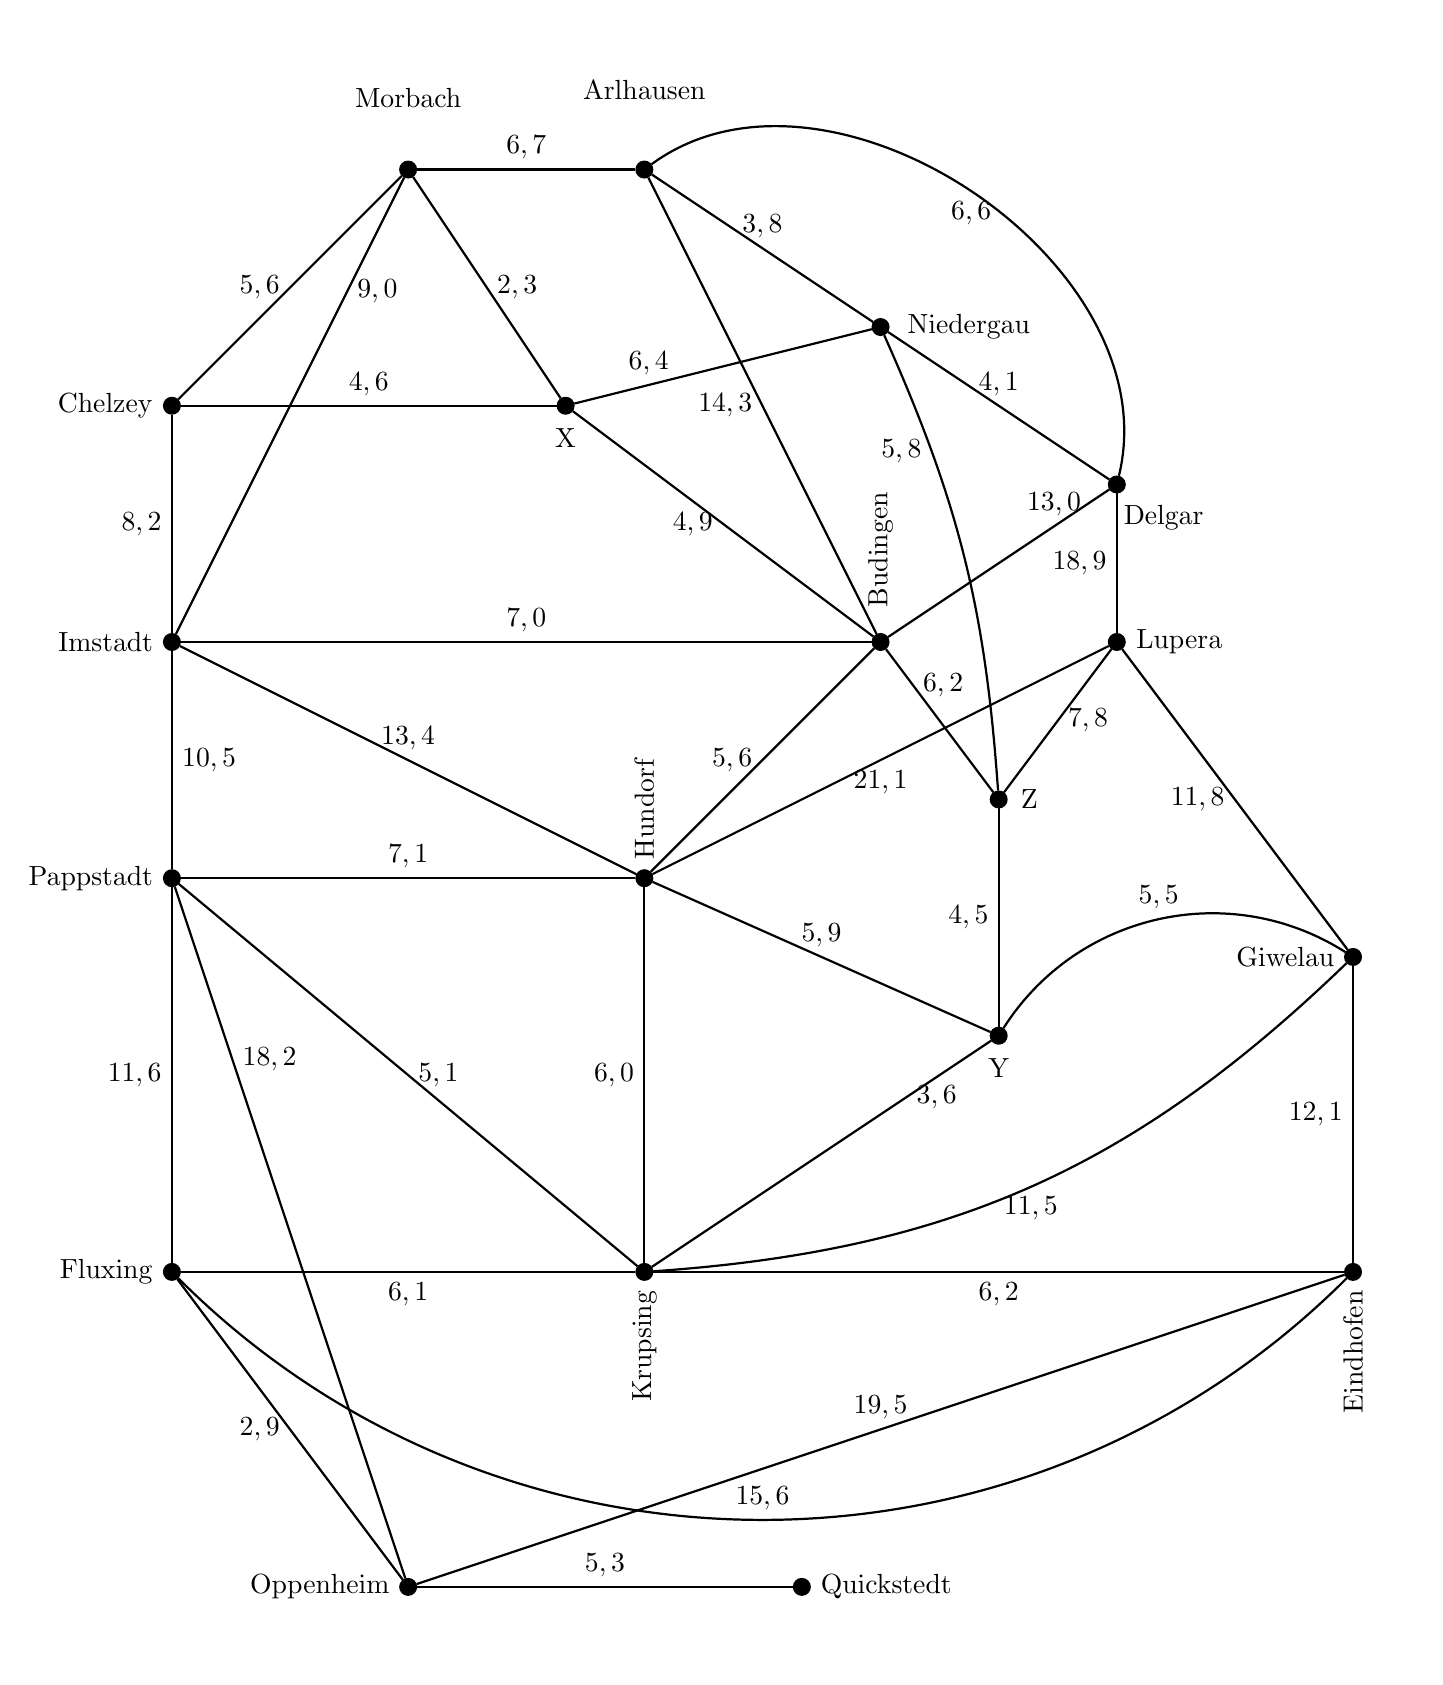
\begin{tikzpicture}
\begin{scope}[every node/.style={circle, thick, fill, draw, inner sep=0cm, minimum size=0.2cm}]
    \node[label={[label distance=0.1cm]180:Imstadt}] (v1) at (-3,0) {};
    \node[label={[label distance=0.1cm]180:Chelzey}] (v2) at (-3,3) {};
    \node[label={[label distance=0.1cm]90:Morbach}] (v3) at (0,6) {};
    \node[label={[label distance=0.1cm]270:X}] (v4) at (2,3) {};
    \node[label={[label distance=0.3cm]90:\rotatebox{90}{Budingen}}] (v5) at (6,0) {};
    \node[label={[label distance=0.1cm]90:\rotatebox{90}{Hundorf}}] (v6) at (3,-3) {};
    \node[label={[label distance=0.1cm]180:Pappstadt}] (v7) at (-3,-3) {};
    \node[label={[label distance=0.1cm]90:Arlhausen}] (v8) at (3,6) {};
    \node[label={[label distance=0.2cm]0:Niedergau}] (v9) at (6,4) {};
    \node[label={[label distance=0.1cm]350:Delgar}] (v10) at (9,2) {};
    \node[label={[label distance=0.1cm]0:Z}] (v11) at (7.5,-2) {};
    \node[label={[label distance=0.1cm]0:Lupera}] (v12) at (9,0) {};
    \node[label={[label distance=0.1cm]180:Giwelau}] (v13) at (12,-4) {};
    \node[label={[label distance=0.1cm]270:Y}] (v14) at (7.5,-5) {};
    \node[label={[label distance=0.1cm]270:\rotatebox{90}{Eindhofen}}] (v15) at (12,-8) {};
    \node[label={[label distance=0.1cm]270:\rotatebox{90}{Krupsing}}] (v16) at (3,-8) {};
    \node[label={[label distance=0.1cm]180:Fluxing}] (v17) at (-3,-8) {};
    \node[label={[label distance=0.1cm]180:Oppenheim}] (v18) at (0,-12) {};
    \node[label={[label distance=0.1cm]0:Quickstedt}] (v19) at (5,-12) {};
\end{scope}
\begin{scope}[every edge/.style={draw=black, thick}]
    \path (v1) edge node[left] {$8,2$} (v2);
    \path (v1) edge node[near end, right] {$9,0$} (v3);
    \path (v1) edge node[above] {$7,0$} (v5);
    \path (v1) edge node[above] {$13,4$} (v6);
    \path (v1) edge node[right] {$10,5$} (v7);
    \path (v2) edge node[left] {$5,6$} (v3);
    \path (v2) edge node[above] {$4,6$} (v4);
    \path (v3) edge node[right] {$2,3$} (v4);
    \path (v3) edge node[above] {$6,7$} (v8);
    \path (v4) edge node[left] {$4,9$} (v5);
    \path (v4) edge node[near start, above] {$6,4$} (v9);
    \path (v5) edge node[left] {$5,6$} (v6);
    \path (v5) edge node[left] {$14,3$} (v8);
    \path (v5) edge node[near end, above] {$13,0$} (v10);
    \path (v5) edge node[near start, right] {$6,2$} (v11);
    \path (v6) edge node[above] {$7,1$} (v7);
    \path (v6) edge node[above] {$5,9$} (v14);
    \path (v6) edge node[left] {$6,0$} (v16);
    \path (v7) edge node[right] {$5,1$} (v16);
    \path (v7) edge node[left] {$11,6$} (v17);
    \path (v7) edge node[right, near start] {$18,2$} (v18);
    \path (v8) edge node[above] {$3,8$} (v9);
    \path (v8) edge[bend left=70, below] node {$6,6$} (v10);
    \path (v9) edge node[above] {$4,1$} (v10);
    \path (v9) edge[bend left=10] node[near start, left] {$5,8$} (v11);
    \path (v10) edge node[left] {$18,9$} (v12);
    \path (v11) edge node[left] {$4,5$} (v14);
    \path (v12) edge node[right] {$7,8$} (v11);
    \path (v12) edge node[left] {$11,8$} (v13);
    \path (v12) edge node[below] {$21,1$} (v6);
    \path (v13) edge node[left] {$12,1$} (v15);
    \path (v13) edge[bend left=20, below] node {$11,5$} (v16);
    \path (v14) edge node[right, near start] {$3,6$} (v16);
    \path (v14) edge[bend left=45, above] node {$5,5$} (v13);
    \path (v15) edge node[below] {$6,2$} (v16);
    \path (v15) edge[bend left=45, above] node {$15,6$} (v17);
    \path (v15) edge node[above] {$19,5$} (v18);
    \path (v16) edge node[below] {$6,1$} (v17);
    \path (v17) edge node[left] {$2,9$} (v18);
    \path (v18) edge node[above] {$5,3$} (v19);
\end{scope}
\end{tikzpicture}
}
\caption{Die Strassenkarte nach der Methode der Gleichformung. Es gibt noch drei Konzepte: Städte, Strassen und Längenangaben.}
\label{figure-graph-strassekarte-2}
\end{figure}

\subsection{Schreibarbeit sparen}

Städtenamen sind \say{mühsam} zum Eintippen. Eigentlich ist es für den Computer egal, wie die Städte heissen. Hauptsache es gibt für jeden Ort, an dem wir die Strasse wechseln können, eine \textbf{eindeutige Bezeichnung}. Wir führen die Bezeichnungen $v_1$, $v_2$, ... , $v_{19}$ ein. Unsere ursprüngliche Fragestellung\footnote{Welches ist der kürzeste Weg von Imstadt nach Oppenheim?} wird nun übersetzt in \say{Welches ist der kürzeste Weg von $v_1$ nach $v_{18}$?}. Wir könnten uns in einer Tabelle \say{merken}, welche Stadt hinter den Bezeichnungen $v_1$, $v_2$, ... stecken und dadurch die ursprüngliche Fragestellung vollständig beantworten. Darauf verzichten wir jedoch, gegebenenfalls \say{erinnern} wir uns wieder an diesen Umstand. Wir erhalten die abschliessende Darstellung in \autoref{figure-graph-strassekarte-3}. Es handelt sich um einen \textbf{gewichteten Graphen}. Diesen können wir leicht in ein Computerprogramm übertragen.

\begin{figure}[htb]
\centering
\resizebox{!}{17cm}{
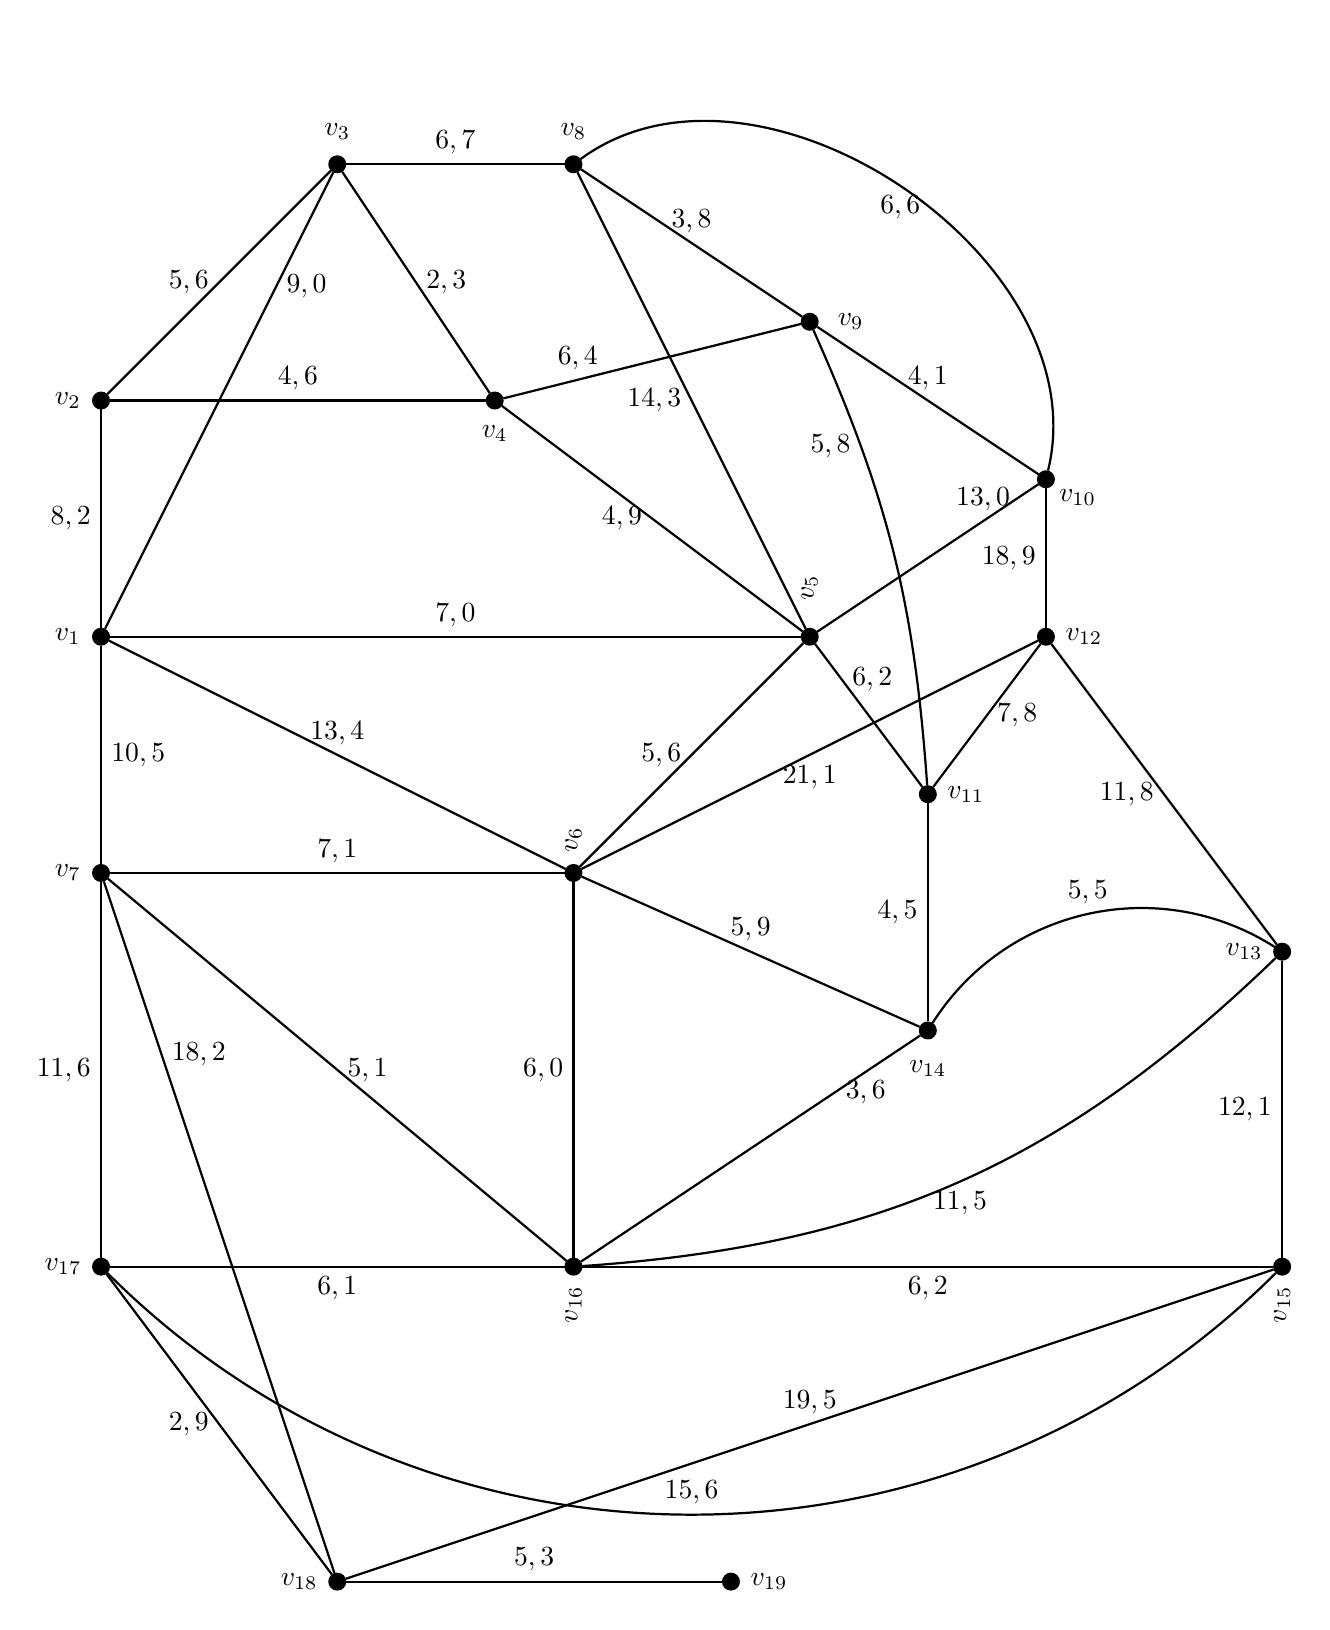
\begin{tikzpicture}
\begin{scope}[every node/.style={circle, thick, fill, draw, inner sep=0cm, minimum size=0.2cm}]
    \node[label={[label distance=0.1cm]180:$v_1$}] (v1) at (-3,0) {};
    \node[label={[label distance=0.1cm]180:$v_2$}] (v2) at (-3,3) {};
    \node[label={[label distance=0.1cm]90:$v_3$}] (v3) at (0,6) {};
    \node[label={[label distance=0.1cm]270:$v_4$}] (v4) at (2,3) {};
    \node[label={[label distance=0.3cm]90:\rotatebox{90}{$v_5$}}] (v5) at (6,0) {};
    \node[label={[label distance=0.1cm]90:\rotatebox{90}{$v_6$}}] (v6) at (3,-3) {};
    \node[label={[label distance=0.1cm]180:$v_7$}] (v7) at (-3,-3) {};
    \node[label={[label distance=0.1cm]90:$v_8$}] (v8) at (3,6) {};
    \node[label={[label distance=0.2cm]0:$v_9$}] (v9) at (6,4) {};
    \node[label={[label distance=0.1cm]350:$v_{10}$}] (v10) at (9,2) {};
    \node[label={[label distance=0.1cm]0:$v_{11}$}] (v11) at (7.5,-2) {};
    \node[label={[label distance=0.1cm]0:$v_{12}$}] (v12) at (9,0) {};
    \node[label={[label distance=0.1cm]180:$v_{13}$}] (v13) at (12,-4) {};
    \node[label={[label distance=0.1cm]270:$v_{14}$}] (v14) at (7.5,-5) {};
    \node[label={[label distance=0.1cm]270:\rotatebox{90}{$v_{15}$}}] (v15) at (12,-8) {};
    \node[label={[label distance=0.1cm]270:\rotatebox{90}{$v_{16}$}}] (v16) at (3,-8) {};
    \node[label={[label distance=0.1cm]180:$v_{17}$}] (v17) at (-3,-8) {};
    \node[label={[label distance=0.1cm]180:$v_{18}$}] (v18) at (0,-12) {};
    \node[label={[label distance=0.1cm]0:$v_{19}$}] (v19) at (5,-12) {};
\end{scope}
\begin{scope}[every edge/.style={draw=black, thick}]
    \path (v1) edge node[left] {$8,2$} (v2);
    \path (v1) edge node[near end, right] {$9,0$} (v3);
    \path (v1) edge node[above] {$7,0$} (v5);
    \path (v1) edge node[above] {$13,4$} (v6);
    \path (v1) edge node[right] {$10,5$} (v7);
    \path (v2) edge node[left] {$5,6$} (v3);
    \path (v2) edge node[above] {$4,6$} (v4);
    \path (v3) edge node[right] {$2,3$} (v4);
    \path (v3) edge node[above] {$6,7$} (v8);
    \path (v4) edge node[left] {$4,9$} (v5);
    \path (v4) edge node[near start, above] {$6,4$} (v9);
    \path (v5) edge node[left] {$5,6$} (v6);
    \path (v5) edge node[left] {$14,3$} (v8);
    \path (v5) edge node[near end, above] {$13,0$} (v10);
    \path (v5) edge node[near start, right] {$6,2$} (v11);
    \path (v6) edge node[above] {$7,1$} (v7);
    \path (v6) edge node[above] {$5,9$} (v14);
    \path (v6) edge node[left] {$6,0$} (v16);
    \path (v7) edge node[right] {$5,1$} (v16);
    \path (v7) edge node[left] {$11,6$} (v17);
    \path (v7) edge node[right, near start] {$18,2$} (v18);
    \path (v8) edge node[above] {$3,8$} (v9);
    \path (v8) edge[bend left=70, below] node {$6,6$} (v10);
    \path (v9) edge node[above] {$4,1$} (v10);
    \path (v9) edge[bend left=10] node[near start, left] {$5,8$} (v11);
    \path (v10) edge node[left] {$18,9$} (v12);
    \path (v11) edge node[left] {$4,5$} (v14);
    \path (v12) edge node[right] {$7,8$} (v11);
    \path (v12) edge node[left] {$11,8$} (v13);
    \path (v12) edge node[below] {$21,1$} (v6);
    \path (v13) edge node[left] {$12,1$} (v15);
    \path (v13) edge[bend left=20, below] node {$11,5$} (v16);
    \path (v14) edge node[right, near start] {$3,6$} (v16);
    \path (v14) edge[bend left=45, above] node {$5,5$} (v13);
    \path (v15) edge node[below] {$6,2$} (v16);
    \path (v15) edge[bend left=45, above] node {$15,6$} (v17);
    \path (v15) edge node[above] {$19,5$} (v18);
    \path (v16) edge node[below] {$6,1$} (v17);
    \path (v17) edge node[left] {$2,9$} (v18);
    \path (v18) edge node[above] {$5,3$} (v19);
\end{scope}
\end{tikzpicture}
}
\caption{Die Strassenkarte wird als gewichteter Graph modelliert.}
\label{figure-graph-strassekarte-3}
\end{figure}

\newpage

\subsection{Aufgaben}

\begin{enumerate}
\item Erstellen Sie für die Strassenkarte aus \autoref{figure-map-ch} den gewichteten Graphen.

\begin{figure}[htb]
\centering
\includegraphics[scale=0.75]{map_ch}
\caption{Auszug aus einer Strassenkarte in der Schweiz (stark vereinfacht).}
\label{figure-map-ch}
\end{figure}

\fillwithgrid	{\stretch{1}}

\newpage

\item Erstellen Sie für die eingezeichneten Fahrradrouten von der Kantonsschule Wettingen zur Kantonsschule Baden aus \autoref{figure-map-kswe} einen ungerichteten Graphen.

\begin{figure}[htb]
\centering
\includegraphics[scale=0.46]{google_maps_kswe_ksb_aufgabe}
\caption{Screenshot der Routenplanung für das Fahrrad.}
\label{figure-map-kswe}
\end{figure}

\fillwithgrid	{\stretch{1}}

\end{enumerate}

\newpage

\section{Kürzester-Weg-Problem}

Wir betrachten also nun folgendes Problem:

\begin{problem}[Kürzester-Weg-Problem]\label{problem-shortest-path}
	Es sind ein gewichteter Graph und zwei Knoten $s$ (Startknoten) und $t$ (Zielknoten) gegeben. Wir suchen nun den \textbf{Weg} von $s$ nach $t$ mit \textbf{minimaler Länge}. Dieses Optimierungsproblem ist in der Informatik als Kürzester-Weg-Problem (eng. \textbf{shortest path problem}) bekannt.
\end{problem}

Bevor wir einen ersten Algorithmus zur Lösung des Problems präsentieren, besprechen wir die Fachbegriffe aus der Definition.

\subsection{Wege}

Wenn wir den kürzesten Weg in einem gewichteten Graphen ermitteln möchten, dann müssen wir wissen, was wir in der Graphentheorie unter einem Weg versteht.

\begin{definition}[Weg]
Ein Weg $p$ (eng. path) ist eine \textbf{Folge von Knoten}, wobei die Knoten, wie bei einer Kette, stets durch eine Kante verbunden sein müssen. Ausserdem darf in der Folge von Knoten \textbf{kein Knoten mehrmals} vorkommen.
\end{definition}

\begin{example}
	Betrachte wir den Graphen aus \autoref{figure-graph-10}. Es gibt etwa folgende Wege:
	\begin{multicols}{3}
	\begin{itemize}
		\item $p_{1}=(v_1, v_2, v_3, v_5)$
		\item $p_{2}=(v_4, v_5, v_6)$
		\item $p_{3}=(v_1, v_2, v_4, v_5, v_6)$
	\end{itemize}
	\end{multicols}
	Der Weg $p_1$ ist farblich hervorgehoben. Eigentlich müssten wir nur die Knoten markieren, aber so können wir den Weg besser erkennen. $p_1$ besitzt den Startknoten $v_1$ und den Zielknoten $v_5$. 

\begin{figure}[htb]
\centering
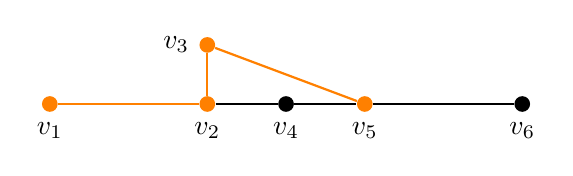
\begin{tikzpicture}
    \node[circle, fill, inner sep=2pt, label={south:$v_1$}, color=orange] (v1) at (0,0) {};
    \node[circle, fill, inner sep=2pt, label={south:$v_2$}, color=orange] (v2) at (2,0) {};
    \node[circle, fill, inner sep=2pt, label={west:$v_3$}, color=orange] (v3) at (2,0.75) {};
    \node[circle, fill, inner sep=2pt, label={south:$v_4$}] (v4) at (3,0) {};
    \node[circle, fill, inner sep=2pt, label={south:$v_5$}, color=orange] (v5) at (4,0) {};
    \node[circle, fill, inner sep=2pt, label={south:$v_6$}] (v6) at (6,0) {};
    \path (v1) edge[color=orange, thick] (v2);
    \path (v2) edge[color=orange, thick] (v3);
    \path (v2) edge[thick] (v4);
    \path (v3) edge[color=orange, thick] (v5);
    \path (v4) edge[thick] (v5);
    \path (v5) edge[thick] (v6);
\end{tikzpicture}
\caption{Der Graph besitzt 6 Knoten und 6 Kanten.}
\label{figure-graph-10}
\end{figure}

Die Knoten $(v_1, v_3, v_5)$ bilden \textbf{keinen Weg}, da zwischen $v_1$ und $v_3$ keine Kante existiert. Auch die Knoten $(v_2, v_3, v_5, v_4, v_2, v_1)$ bilden \textbf{keinen Weg}, da $v_2$ zweimal vorkommt.
\end{example}

\subsection{Länge eines Wegs}

In einem gewichteten Graphen können wir die Länge eines Wegs bestimmen.

\begin{definition}[Länge eines Wegs]
	In einem gewichteten Graphen $G = (E, V, w)$ können wir die Länge eines Wegs $p$ berechnen, in dem wir die Gewichte der Kanten von $p$ addieren. Wir bezeichnen die Länge eines Wegs $p$ mit $l(p)$.
\end{definition}

\begin{example}
	Wir berechnen die Länge für den Weg $p = (v_1, v_2, v_3)$ aus \autoref{figure-graph-12} in dem wir die Gewichte für die Kanten addieren:
\begin{align*}
	l(p) = l((v_1, v_2, v_3)) = w(\{v_1, v_2\}) + w(\{v_2, v_3\}) = 2 + 42 = 44
\end{align*}

\begin{figure}[htb]
\centering
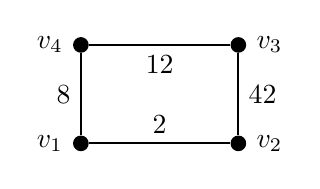
\begin{tikzpicture}
    \node[circle, fill, inner sep=2pt, label={west:$v_1$}] (v1) at (0,0) {};
    \node[circle, fill, inner sep=2pt, label={east:$v_2$}] (v2) at (2,0) {};
    \node[circle, fill, inner sep=2pt, label={east:$v_3$}] (v3) at (2,1.25) {};
    \node[circle, fill, inner sep=2pt, label={west:$v_4$}] (v4) at (0,1.25) {};
    
    \path[thick] (v1) edge node[above] {$2$} (v2);
    \path[thick] (v2) edge node[right] {$42$} (v3);
    \path[thick] (v3) edge node[below] {$12$} (v4);
    \path[thick] (v4) edge node[left] {$8$} (v1);
\end{tikzpicture}
\caption{Der Graph besitzt 4 Knoten und 4 Kanten.}
\label{figure-graph-12}
\end{figure}
\end{example}

\subsection{Kürzester Weg}

Wir haben alle Begriffe geklärt, um den kürzesten Weg in einem gewichteten Graphen zu definieren.

\begin{definition}[Kürzester Weg]
Der kürzeste Weg zwischen einem Startknoten $s$ und einem Zielknoten $t$ ist derjenige Weg von $s$ nach $t$ mit \textbf{minimaler Länge}. Die Länge des kürzesten Wegs bezeichnen wir als \textbf{Distanz} und wird mit $d(s, t)$ notiert. 
\end{definition}

\begin{important}
Wir lösen in den folgenden Abschnitten das Kürzester-Weg-Problem für \textbf{Distanzgraphen}.
\end{important}

\subsection{Aufgaben}

Beantworten Sie die folgenden Fragen bezüglich des Graphen aus \autoref{figure-graph-11}.

\begin{enumerate}
	\item Markieren Sie den Weg $p=(v_1, v_4, v_2, v_5, v_3)$ im Graphen.
	\item Notieren Sie einen anderen Weg mit $5$ Knoten.
	\item Notieren Sie alle Wege von $v_1$ nach $v_3$ mit maximal $4$ Knoten.
	\item Ist $p=(v_1, v_3, v_2, v_4)$ ein Weg? Begründen Sie Ihre Antwort.

\begin{figure}[htb]
\centering
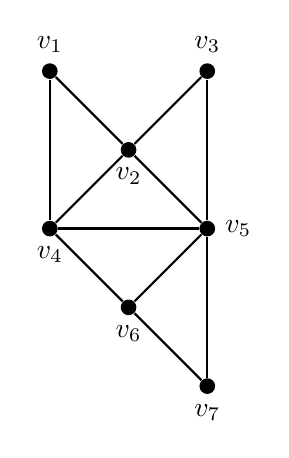
\begin{tikzpicture}
    \node[circle, fill, inner sep=2pt, label={north:$v_1$}] (v1) at (0,0) {};
    \node[circle, fill, inner sep=2pt, label={south:$v_2$}] (v2) at (1,-1) {};
    \node[circle, fill, inner sep=2pt, label={north:$v_3$}] (v3) at (2,0) {};
    \node[circle, fill, inner sep=2pt, label={south:$v_4$}] (v4) at (0,-2) {};
    \node[circle, fill, inner sep=2pt, label={east:$v_5$}] (v5) at (2,-2) {};
    \node[circle, fill, inner sep=2pt, label={south:$v_6$}] (v6) at (1,-3) {};
    \node[circle, fill, inner sep=2pt, label={south:$v_7$}] (v7) at (2,-4) {};
    \path (v1) edge[thick] (v2);
    \path (v1) edge[thick] (v4);
    \path (v2) edge[thick] (v3);
    \path (v2) edge[thick] (v4);
    \path (v2) edge[thick] (v5);
    \path (v3) edge[thick] (v5);
    \path (v4) edge[thick] (v5);
    \path (v4) edge[thick] (v6);
    \path (v5) edge[thick] (v6);
    \path (v5) edge[thick] (v7);
    \path (v6) edge[thick] (v7);
\end{tikzpicture}
\caption{Der Graph besitzt 7 Knoten und 11 Kanten.}
\label{figure-graph-11}
\end{figure}

\fillwithgrid{\stretch{1}}

\newpage

\item Berechnen Sie die Länge von $p = (v_1, v_4, v_3)$ aus dem Graph aus \autoref{figure-aufgaben-graph-2}. Notieren Sie alle Rechenschritte wie im Beispiel.

\begin{figure}[htb]
\centering
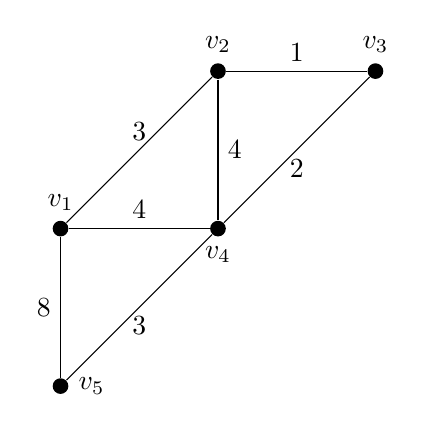
\begin{tikzpicture}
    \node[circle, fill, inner sep=2pt, label={north:$v_1$}] (v1) at (0,0) {};
    \node[circle, fill, inner sep=2pt, label={north:$v_2$}] (v2) at (2,2) {};
    \node[circle, fill, inner sep=2pt, label={north:$v_3$}] (v3) at (4,2) {};
    \node[circle, fill, inner sep=2pt, label={south:$v_4$}] (v4) at (2,0) {};
    \node[circle, fill, inner sep=2pt, label={east:$v_5$}] (v5) at (0,-2) {};
    \path (v1) edge node[above] {$3$} (v2);
    \path (v1) edge node[above] {$4$} (v4);
    \path (v1) edge node[left] {$8$} (v5);
    \path (v2) edge node[above] {$1$}  (v3);
    \path (v2) edge node[right] {$4$}  (v4);
    \path (v3) edge node[below] {$2$}  (v4);
    \path (v4) edge node[below] {$3$}  (v5);
\end{tikzpicture}
\caption{Der Graph besitzt 5 Knoten und 7 Kanten.}
\label{figure-aufgaben-graph-2}
\end{figure}

\fillwithgrid{2in}

\item Berechnen Sie die Länge von $p = (v_1, v_2, v_3, v_4, v_5)$ aus dem Graph aus \autoref{figure-aufgaben-graph-2}. Notieren Sie alle Rechenschritte wie im Beispiel.

\fillwithgrid{\stretch{1}}

\end{enumerate}

\newpage

\section{Alle-Wege-Ausprobieren-Algorithmus}

Wir können einen ersten, sehr einfachen Algorithmus formulieren, welcher den kürzesten Weg zwischen einem Startknoten und einem Zielknoten ermittelt.

\begin{lstlisting}[language={pseudocode}, caption={Ein Brute-Force-Algorithmus für das Kürzeste-Weg-Problem.}, label={lst-algo-shortest-path-brute-force}]
input: Graph G = (V, E, w), Startknoten s, Zielknoten t.

1.) Liste alle Wege von s nach t auf.
2.) Berechne für alle Wege aus 1.) die Länge.
3.) Vergleiche die Längen der Wege. Wähle denjenigen Weg 
    mit minimaler Länge aus. Gibt es mehrere Wege mit 
    gleicher Länge, dann wähle irgendeinen Weg aus.
    Dies ist der kürzeste Weg p_min. 
  
output: p_min.
\end{lstlisting}

Der Algorithmus aus \autoref{lst-algo-shortest-path-brute-force} löst das Kürzester-Weg-Problem (siehe Problem \autoref{problem-shortest-path}). Wir führen den Algorithmus an einem Beispiel aus.

\begin{example}
	Es sei der Graph aus \autoref{figure-graph-13} gegeben. Wir möchten den kürzesten Weg von $s = v_1$ nach $t = v_6$ bestimmen.

\begin{figure}[ht]
\centering
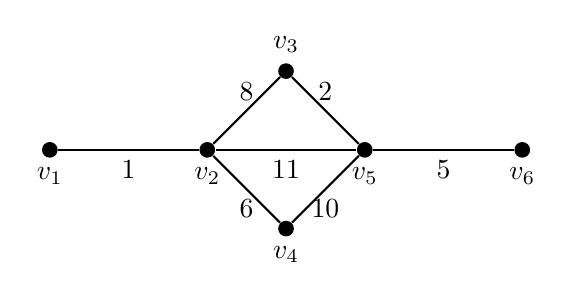
\begin{tikzpicture}
    \node[circle, fill, inner sep=2pt, label={south:$v_1$}] (v1) at (0,0) {};
    \node[circle, fill, inner sep=2pt, label={south:$v_2$}] (v2) at (2,0) {};
    \node[circle, fill, inner sep=2pt, label={north:$v_3$}] (v3) at (3,1) {};
    \node[circle, fill, inner sep=2pt, label={south:$v_4$}] (v4) at (3,-1) {};
    \node[circle, fill, inner sep=2pt, label={south:$v_5$}] (v5) at (4,0) {};
    \node[circle, fill, inner sep=2pt, label={south:$v_6$}] (v6) at (6,0) {};
    \path[thick] (v1) edge node[below] {$1$} (v2);
    \path[thick] (v2) edge node[above] {$8$} (v3);
    \path[thick] (v2) edge node[below] {$6$} (v4);
    \path[thick] (v2) edge node[below] {$11$} (v5);
    \path[thick] (v3) edge node[above] {$2$} (v5);
    \path[thick] (v4) edge node[below] {$10$} (v5);
    \path[thick] (v5) edge node[below] {$5$} (v6);
\end{tikzpicture}
\caption{Graph mit $6$ Knoten und $7$ Kanten.}
\label{figure-graph-13}
\end{figure}

\begin{itemize}
	\item Schritt 1: Alle Wege von $v_1$ nach $v_6$ auflisten.
	\begin{itemize}
		\item $p_1 = (v_1, v_2, v_3, v_5, v_6)$
		\item $p_2 = (v_1, v_2, v_5, v_6)$
		\item $p_3 = (v_1, v_2, v_4, v_5, v_6)$
	\end{itemize}	
	\item Schritt 2: Länge der Wege aus Schritt 1 berechnen.
	\begin{itemize}
		\item $l(p_1) = 1 + 8 + 2 + 5 = 16$
		\item $l(p_2) = 1 + 11 + 5 = 17$
		\item $l(p_3) = 1 + 6 + 10 + 5 = 22$
	\end{itemize}
	\item Schritt 3: Weg mit minimaler Länge auswählen: $\underset{i}{\mathrm{arg~min}}~l(p_i) = 1 \Rightarrow p_{min} = p_1$.
\end{itemize}

Der Weg $p_1$ mit einer Länge von $16$ ist somit der kürzeste Weg. Die Distanz von $v_1$ und $v_6$ ist somit $d(v_1, v_6) = 16$.

\end{example}

Wir haben einen Algorithmus gefunden, der den kürzesten Weg zwischen zwei Knoten bestimmen kann. Wir können die Schritte durchführen und erhalten den kürzesten Weg. Das Prinzip des Algorithmus ist es, alle möglichen Wege zu ermitteln und dann den kürzesten Weg auszuwählen. Deshalb nennen wir diesen Algorithmus \textbf{Alle-Wege-Ausprobieren-Algorithmus}.

Algorithmen, die zur Lösung eines Problems alle Möglichkeiten ausprobieren und dann die \say{beste} auswählen, bezeichnen wir als \textbf{Brute-Force-Algorithmen}. Die Brute-Force-Algorithmen funktionieren in der Theorie, müssen jedoch auch in der Praxis effizient arbeiten. In einem anderen Abschnitt klären wir die Praxistauglichkeit des Alle-Wege-Ausprobieren-Algorithmus.

\subsection{Aufgaben}
\label{subsection-aufgaben-routenplaner-brute-force}

\begin{enumerate}
	\item Berechnen Sie den kürzesten Weg von $v_1$ nach $v_3$ für den Graphen aus \autoref{figure-graph-15} mithilfe des Alle-Wege-Ausprobieren-Algorithmus.
	
\begin{figure}[htb]
\centering
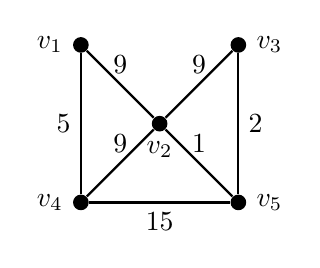
\begin{tikzpicture}
    \node[circle, fill, inner sep=2pt, label={west:$v_1$}] (v1) at (0,0) {};
    \node[circle, fill, inner sep=2pt, label={south:$v_2$}] (v2) at (1,-1) {};
    \node[circle, fill, inner sep=2pt, label={east:$v_3$}] (v3) at (2,0) {};
    \node[circle, fill, inner sep=2pt, label={west:$v_4$}] (v4) at (0,-2) {};
    \node[circle, fill, inner sep=2pt, label={east:$v_5$}] (v5) at (2,-2) {};
    \path (v1) edge[thick] node[above] {$9$} (v2);
    \path (v1) edge[thick] node[left] {$5$} (v4);
    \path (v2) edge[thick] node[above] {$9$} (v3);
    \path (v2) edge[thick] node[above] {$9$} (v4);
    \path (v2) edge[thick] node[above] {$1$} (v5);
    \path (v3) edge[thick] node[right] {$2$} (v5);
    \path (v4) edge[thick] node[below] {$15$} (v5);
\end{tikzpicture}
\caption{Der Graph besitzt $5$ Knoten und $7$ Kanten.}
\label{figure-graph-14}
\end{figure}

\fillwithgrid{1.75in}

	\item Berechnen Sie den kürzesten Weg von $v_1$ nach $v_9$ für den Graphen aus \autoref{figure-graph-15} mithilfe des Alle-Wege-Ausprobieren-Algorithmus.

\begin{figure}[htb]
\centering
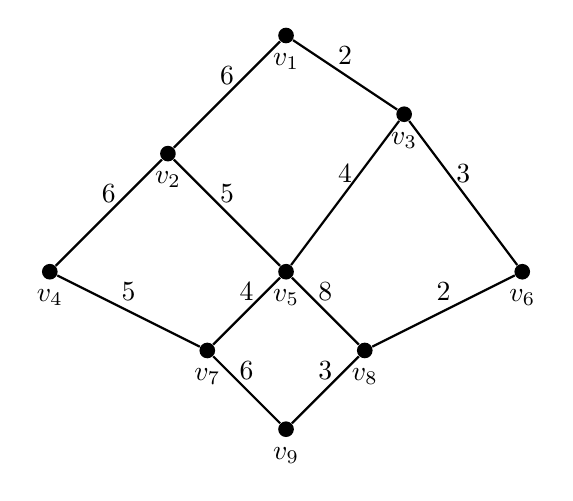
\begin{tikzpicture}
    \node[circle, fill, inner sep=2pt, label={south:$v_1$}] (v1) at (0,0) {};
    \node[circle, fill, inner sep=2pt, label={south:$v_2$}] (v2) at (-1.5,-1.5) {};
    \node[circle, fill, inner sep=2pt, label={south:$v_3$}] (v3) at (1.5,-1) {};
    \node[circle, fill, inner sep=2pt, label={south:$v_5$}] (v5) at (0,-3) {};
    \node[circle, fill, inner sep=2pt, label={south:$v_4$}] (v4) at (-3,-3) {};
    \node[circle, fill, inner sep=2pt, label={south:$v_6$}] (v6) at (3,-3) {};
    \node[circle, fill, inner sep=2pt, label={south:$v_7$}] (v7) at (-1,-4) {};
    \node[circle, fill, inner sep=2pt, label={south:$v_8$}] (v8) at (1,-4) {};
    \node[circle, fill, inner sep=2pt, label={south:$v_9$}] (v9) at (0,-5) {};
    \path (v1) edge[thick] node[above] {$6$} (v2);
    \path (v1) edge[thick] node[above] {$2$} (v3);
    \path (v2) edge[thick] node[above] {$5$} (v5);
    \path (v2) edge[thick] node[above] {$6$} (v4);
    \path (v3) edge[thick] node[above] {$4$} (v5);
    \path (v3) edge[thick] node[above] {$3$} (v6);
    \path (v4) edge[thick] node[above] {$5$} (v7);
    \path (v5) edge[thick] node[above] {$4$} (v7);
    \path (v6) edge[thick] node[above] {$2$} (v8);
    \path (v5) edge[thick] node[above] {$8$} (v8);
    \path (v7) edge[thick] node[above] {$6$} (v9);
    \path (v8) edge[thick] node[above] {$3$} (v9);
\end{tikzpicture}
\caption{Der Graph besitzt $9$ Knoten und $12$ Kanten.}
\label{figure-graph-15}
\end{figure}

\fillwithgrid{\stretch{1}}

\newpage

\end{enumerate}

\section{Laufzeitanalyse des Alle-Wege-Ausprobieren-Algorithmus}

Können wir den Alle-Wege-Ausprobieren-Algorithmus in der Praxis einsetzen? Wir müssen die Antwort auf diese Frage für einen grösseren Graphen mit mehreren tausend Knoten ermitteln. Nur so wissen wir, ob der Algorithmus in der Praxis etwas taugt. Wir müssen also die \textbf{asymptotische Laufzeit des Algorithmus im schlechtesten Fall} bestimmen, das heisst $T_{\text{WC}}$.

\subsection{Worst-Case-Laufzeit}

 Wir möchten die asymptotische Worst-Case-Laufzeit $T_{\text{WC}}$ gerne in \textbf{Abhängigkeit} von der \textbf{Grösse des Graphen} angeben. Wir messen dabei die Grösse des Graphen durch die Anzahl der Knoten. Da wir an $T_{\text{WC}}$ interessiert sind, möchten wir die \textbf{Anzahl der Wege} im Graphen mit $n$ Knoten \textbf{maximieren}. Dies erreichen wir, in dem jeder Knoten mit jedem anderen Knoten verbunden ist. 

\begin{definition}[Vollständiger Graph mit $n$ Knoten]
	Ein vollständiger Graph mit $n$ Knoten (eng. complete graph) wird mit $K_n$ abgekürzt und besitzt $\frac{n\cdot(n-1)}{2}$ Kanten.
\end{definition}

\autoref{figure-complete-graphs} zeigt drei Beispiele. Vollständige Graphen gibt es für eine beliebige Anzahl von Knoten. Damit die Graphen übersichtlich bleiben, verzichten wir auf Gewichte. Bei der folgenden Analyse gehen wir jedoch davon aus, dass jede Kante ein Gewicht besitzt.

\begin{figure}[htb]
	\centering
	\begin{minipage}{0.3\textwidth}
		\begin{tikzpicture}
		\graph[nodes={circle, fill, inner sep=2pt}, n=5, radius=1.5cm, clockwise, empty nodes] { 1[label={north:$v_1$}]; 2[label={east:$v_2$}]; 3[label={south:$v_3$}]; 4[label={south:$v_4$}]; 5[label={west:$v_5$}]; subgraph K_n };
		\end{tikzpicture}
	\end{minipage}
	\begin{minipage}{0.3\textwidth}
		\begin{tikzpicture}
		\graph[nodes={circle, fill, inner sep=2pt}, n=6, radius=1.5cm, clockwise, empty nodes] { 1[label={north:$v_1$}]; 2[label={east:$v_2$}]; 3[label={east:$v_3$}]; 4[label={south:$v_4$}]; 5[label={west:$v_5$}]; 6[label={west:$v_6$}]; subgraph K_n };
		\end{tikzpicture}
	\end{minipage}
	\begin{minipage}{0.3\textwidth}
	\begin{tikzpicture}
		\graph[nodes={circle, fill, inner sep=2pt}, n=7, radius=1.5cm, clockwise, empty nodes] { 1[label={north:$v_1$}]; 2[label={east:$v_2$}]; 3[label={east:$v_3$}]; 4[label={east:$v_4$}]; 5[label={west:$v_5$}]; 6[label={west:$v_6$}]; 7[label={west:$v_7$}]; subgraph K_n };
		\end{tikzpicture}
	\end{minipage}
	\caption{Die vollständigen Graphen $K_5$, $K_6$ und $K_7$.}
	\label{figure-complete-graphs}
\end{figure}

Als \textbf{Elementaroperation} wählen wir nun die \textbf{Berechnung der Länge eines Wegs} $p$, das heisst $l(p)$. Für die Worst-Case-Laufzeit müssen wir also herausfinden, wie viele Wege es in einem \textbf{vollständigen Graphen} $K_n$ gibt, denn pro Weg berechnen wir einmal die Länge.
\begin{align*}
T_{\text{WC}}(n) = \text{Anzahl der Wege von s nach t in Abhängigkeit von } n
\end{align*}
Wir fixieren die zwei gegebene Knoten $s$ und $t$. Dann berechnen wir die Anzahl der Wege von $s$ nach $t$ wie folgt:
\begin{align*}
T_{\text{WC}}(n) & = \text{Anzahl der s-t-Wege der Länge 1} + \text{Anzahl der s-t-Wege der Länge 2} \\ & + \text{Anzahl der s-t-Wege der Länge 3} + \cdots + \text{Anzahl der s-t-Wege der Länge } n-1 \\ & = \sum_{k=0}^{n-2}\frac{(n-2)!}{(n-2-k)!} \approx 3\cdot(n-2)!
\end{align*}

Bereits bei $K_{20}$, dass heisst bei \num{20} Knoten, erhalten wir circa \num{7298706024529920000} Wege. Das sind über \num{7} Trillionen Wege. Falls der Computer \num{1} Million Wege pro Sekunde bearbeiten kann, dann benötigt der Computer über \num{231440} Jahre.

\subsection{Zusammenfassung}

Der Alle-Wege-Ausprobieren-Algorithmus besitzt eine \textbf{asymptotische Worst-Case-Laufzeit $T_{\text{WC}}(n)\approx 3\cdot(n-2)!$}. Die Anzahl der Wege wächst also \textbf{faktoriell} mit der \textbf{Anzahl der Knoten} im \textbf{vollständigen Graph}. Dieser Brute-Force-Algorithmus ist also \textbf{kein} Algorithmus, welcher in der Praxis für das Kürzester-Weg-Problem eingesetzt werden kann.

\section{Der Dijkstra-Algorithmus}

Der Algorithmus von Dijkstra berechnet \textbf{schrittweise} den kürzesten Weg zwischen einem Startknoten $s$ und einem Zielknoten $t$. Es ist kein Brute-Force-Algorithmus, da er nicht alle Kombinationen vom Startknoten $s$ zum Zielknoten $t$ ausprobiert werden. \autoref{figure-dijkstra-bsp} zeigt einen Graphen und eine \textbf{Momentaufnahme} des Algorithmus. Bisher wurde nur der kürzeste Weg von $v_1$ nach $v_3$ berechnet (grüne Knoten). Für einen violetten Knoten wird als Nächstes der kürzeste Weg nach $v_1$ berechnet. Die blauen Knoten werden erst später betrachtet.

\begin{figure}[htb]
\centering
\begin{tikzpicture}
    \node[circle, fill, inner sep=2pt, label={[darkgreen]south:$v_1$}, color=darkgreen, label={[darkgreen]north:\textbf{0}}] (v1) at (0,0) {};
    \node[circle, fill, inner sep=2pt, label={[violet]north:$v_2$}, label={[violet]south east:\textbf{4}}, color=violet] (v2) at (2,2) {};
    \node[circle, fill, inner sep=2pt, label={[darkgreen]north east:$v_3$}, label={[darkgreen]north west:\textbf{3}}, color=darkgreen] (v3) at (2,0) {};
    \node[circle, fill, inner sep=2pt, label={[violet]south:$v_4$}, color=violet, label={[violet]north east:\textbf{8}}] (v4) at (2,-2) {};
    
    \node[circle, fill, inner sep=2pt, label={north:$v_5$}, label={[blue]south west:\textbf{$\infty$}}] (v5) at (4,2) {};
    \node[circle, fill, inner sep=2pt, label={[violet]north east:$v_6$}, color=violet, label={[violet]north west:\textbf{12}}] (v6) at (4,0) {};
    \node[circle, fill, inner sep=2pt, label={south:$v_7$}, label={[blue]south east:\textbf{$\infty$}}] (v7) at (4,-2) {};
    
    \node[circle, fill, inner sep=2pt, label={north:$v_8$}, label={[blue]south east:\textbf{$\infty$}}] (v8) at (6,0) {};
    
    \path[thick] (v1) edge node[above] {$5$} node[violet, above, near end, thick, sloped] {$\leftarrow$} (v2);
    \path[thick] (v1) edge node[below] {$3$} node[darkgreen, below, near end, thick] {$\leftarrow$} (v3);
    
    \path[thick] (v1) edge node[below] {$8$} node[violet, below, near end, thick, sloped] {$\leftarrow$} (v4);
    
    \path[thick] (v2) edge node[above] {$3$} (v5);
    \path[thick] (v2) edge node[right] {$1$} (v3);
    \path[thick] (v3) edge node[below] {$9$} node[violet, below, near end, thick, sloped] {$\leftarrow$} (v6);
    \path[thick] (v3) edge node[right] {$11$} (v4);
    \path[thick] (v4) edge node[below] {$1$} (v7);
    
    \path[thick] (v5) edge node[above] {$5$} (v8);
    \path[thick] (v5) edge node[right] {$5$} (v6);
    \path[thick] (v6) edge node[below] {$20$} (v8);
    \path[thick] (v6) edge node[right] {$1$} (v7);
    \path[thick] (v7) edge node[below] {$2$} (v8);
    
    \begin{pgfonlayer}{background}
        \draw[rounded corners=2em, line width=3em, green!30, cap=round] (v1.center) -- (v3.east);
    \end{pgfonlayer}
    
    \begin{pgfonlayer}{background}
        \draw[rounded corners=2em, line width=2.25em, violet!30, cap=round] (v2.center) -- (v6.east) -- (v4.center);
    \end{pgfonlayer}
    
    \begin{pgfonlayer}{background}
        \draw[rounded corners=2em, line width=2.75em, blue!30, cap=round] (v5.center) -- (v8.east) -- (v7.center);
    \end{pgfonlayer}
    
\end{tikzpicture}
\caption{Gewählte Knoten (grün), Randknoten (violett) und unerreichte Knoten (blau).}
\label{figure-dijkstra-bsp}
\end{figure}

Die Einteilung der Knoten in die drei farbigen Gruppen\footnote{Die Farbe ist völlig willkürlich gewählt und kann beliebig ersetzt werden.} zeigt die schrittweise Berechnung der Lösung. Die Einteilung der Knoten in die drei Gruppen ist nicht fix, sondern ändert sich während der Ausführung des Algorithmus.

\subsection{Gruppeneinteilung}

Es gibt drei Gruppen: gewählte Knoten, Randknoten und unerreichte Knoten. Nicht immer muss in jeder Gruppe ein Knoten vorkommen.

\subsubsection{Gewählte Knoten}

Für einen gewählten Knoten $v_i$ steht der kürzeste Weg zum Startknoten $s$ bereits fest und ändert sich nicht mehr. Wir markieren diesen Knoten grün und schreiben die Distanz zum Startknoten in grüner Farbe neben den Knoten. Ausserdem notieren wir mit einem grünen Pfeil diejenige Kante, die zum nächsten grünen Knoten führt.

\begin{important}[Einmal gewählt, immer gewählt]
	Gewählte Knoten bleiben gewählt. Der kürzeste Weg zum Startknoten für alle gewählten Knoten steht fest und ändert sich nicht mehr.
\end{important}

\begin{example}
	In \autoref{figure-dijkstra-bsp} sind $v_1$ und $v_3$ gewählte Knoten. Sie haben die Distanz $0$ und $3$ zum Startknoten. Dies ändert sich \textbf{nicht} mehr.
\end{example}

\subsubsection{Randknoten}

Jeder Randknoten besitzt mindestens eine Kante zu einem gewählten Knoten. Wir markieren jeden Randknoten violett und schreiben die aktuelle Distanz in violetter Farbe zum Startknoten. Ausserdem notieren wir mit einem violetten Pfeil diejenige Kante, die zum grünen Knoten führt. Randknoten können ihre \say{Meinung} noch ändern. Die Distanz und der Pfeil ändern sich gegebenenfalls im Verlauf des Algorithmus.

\begin{important}[Kürzester Weg noch nicht fix]
	Der kürzeste Weg von einem Randknoten zum Startknoten kann sich noch ändern.
\end{important}

\begin{example}
	In \autoref{figure-dijkstra-bsp} sind $v_2$, $v_4$ und $v_6$ Randknoten. Sie haben die Distanz $4$, $12$ und $8$ zum Startknoten. Diese Distanzen können sich noch ändern. Der Knoten $v_6$ besitzt aktuell eine Distanz von $12$ zum Startknoten $v_1$. Es gibt jedoch einen kürzeren Weg mit Distanz $10$. Der Algorithmus wird diesen Weg erst noch \say{entdecken}.
\end{example}

\subsubsection{Unerreichte Knoten}

Zu Beginn des Dijkstra-Algorithmus sind alle Knoten unerreicht. Für einen unerreichten Knoten kennen wir noch keinen Weg zum Startknoten $s$. Ein unerreichter Knoten muss zuerst zu einem Randknoten werden. Dies geschieht immer nur dann, wenn ein Randknoten zu einem gewählten Knoten wird. Unerreichte Knoten markieren wir in blauer Farbe und besitzen eine \say{unendliche} Distanz zum Startknoten.

\begin{example}
	In \autoref{figure-dijkstra-bsp} sind $v_5$, $v_7$ und $v_8$ die drei unerreichten Knoten. Alle Knoten besitzen eine unendliche Distanz. Dies soll verdeutlichen, dass es noch keinen Weg zum Startknoten gibt. Deshalb sind auch keine Pfeile eingezeichnet.
\end{example}

\begin{important}[Unerreichter Knoten $\Rightarrow$ Randknoten $\Rightarrow$ Gewählter Knoten]
	Alle Knoten sind zu Beginn unerreicht. Der Startknoten ist der erste gewählte Knoten. Dann werden die Randknoten erzeugt. Erst dann wird Schritt-für-Schritt jeder unerreichte Knoten \say{entdeckt} und zu einem Randknoten.
\end{important}

\subsection{Algorithmusstrategie}

Der Dijkstra-Algorithmus wählt in jedem Schritt denjenigen Knoten aus den Randknoten aus, der die \textbf{minimale Distanz zum Startknoten} besitzt. Dadurch können wir schrittweise bestehende kürzeste Wege verlängern. Der kürzeste Weg wird gewissermassen Zug um Zug vom Startknoten zum Zielknoten ausgebaut. 

\begin{important}
	Man kann beweisen, dass durch das Hinzufügen der korrekten Kante, der \say{neue} kürzeste Weg weiterhin korrekt bleibt. Wir \say{verpassen} also durch dieses Schritt-für-Schritt-Vorgehen keinen noch kürzeren Weg.
\end{important}

\begin{definition}[Graphenalgorithmus]
	Ein Graphenalgorithmus besitzt als Input einen \textbf{Graphen} und löst ein Problem, welches in Verbindung mit dem Graphen steht.
\end{definition}

\begin{definition}[Greedy-Algorithmus]
Bei einem Greedy-Algorithmus werden gewisse \textbf{Entscheidungen} hinsichtlich der Lösung getroffen und anschliessend \textbf{nicht} mehr revidiert.
\end{definition}

Der Dijkstra-Algorithmus ist ein \textbf{Graphen-} und \textbf{Greedy-Algorithmus}. Wird beim Dijkstra-Algorithmus ein Knoten zum gewählten Knoten, dann wird diese Entscheidung nicht mehr angepasst. Dies ist das \say{Greedy-Verhalten} des Dijkstra-Algorithmus.

\rule{5cm}{0.4pt}

\begin{figure}[htb]
\centering
\begin{minipage}[c]{0.25\textwidth}
\includegraphics[scale=0.09]{dijkstra}
\end{minipage}
\begin{minipage}[c]{0.7\textwidth}
\paragraph{Aus der Informatik-Geschichte...} Edsger Wybe Dijkstra (11. Mai 1930 in Rotterdam, 6. August 2002 in Nuenen) war ein niederländischer Informatiker. Er war der Wegbereiter der strukturierten Programmierung. 1972 erhielt er den Turing Award für grundlegende Beiträge zur Entwicklung von Programmiersprachen. Unter seinen Beiträgen zur Informatik befindet sich der Dijkstra-Algorithmus zur Berechnung des kürzesten Wegs in einem Graphen (1959 in einem dreiseitigen Artikel veröffentlicht \cite{dijkstra-paper-shortest-path}). Das Bild stammt aus dem Jahr 2002.
\end{minipage}
\end{figure}

\subsection{Nachbarschaft}

Der Dijkstra-Algorithmus muss wiederholt die Nachbarschaft (eng. neighbourhood) eines Knotens bestimmen.

\begin{definition}[Nachbarschaft]
Die Nachbarschaft eines Knotens $v_i$ in einem ungerichteten Graphen sind alle Knoten, die mit $v_i$ durch \textbf{eine Kante} verbunden sind. Wir bezeichnen die Nachbarschaft von $v_i$ mit $N(v_i)$. Die Knoten, die in der Nachbarschaft zu $v_i$ sind, werden auch \textbf{Nachbarn} genannt.
\end{definition}

\begin{example}
Der Knoten $v_1$ im ungerichteten Graph aus \autoref{figure-graph-16} besitzt die Nachbarn $v_2$ und $v_3$. Wir können dies formal durch $N(v_1) = \{v_2, v_3 \}$ ausdrücken.

\begin{figure}[htb]
\centering
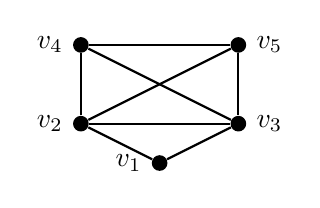
\begin{tikzpicture}
    \node[circle, fill, inner sep=2pt, label={west:$v_1$}] (v1) at (0,0.5) {};
    \node[circle, fill, inner sep=2pt, label={west:$v_2$}] (v2) at (-1,1) {};
    \node[circle, fill, inner sep=2pt, label={east:$v_3$}] (v3) at (1,1) {};
    \node[circle, fill, inner sep=2pt, label={west:$v_4$}] (v4) at (-1,2) {};
    \node[circle, fill, inner sep=2pt, label={east:$v_5$}] (v5) at (1,2) {};
    \path[thick] (v1) edge (v2);
    \path[thick] (v1) edge (v3);
    \path[thick] (v2) edge (v3);
    \path[thick] (v2) edge (v4);
    \path[thick] (v2) edge (v5);
    \path[thick] (v3) edge (v4);
    \path[thick] (v3) edge (v5);
    \path[thick] (v4) edge (v5);
\end{tikzpicture}
\caption{Ein ungerichteter Graph mit 5 Knoten und 8 Kanten.}
\label{figure-graph-16}
\end{figure}

Die Nachbarschaft der anderen Knoten:

\begin{multicols}{2}
\begin{itemize}
	\item $N(v_2) = \{v_1, v_3, v_4, v_5 \}$
	\item $N(v_3) = \{v_1, v_2, v_4, v_5 \}$
	\item $N(v_4) = \{v_2, v_3, v_5 \}$
	\item $N(v_5) = \{v_2, v_3, v_4 \}$
\end{itemize}
\end{multicols}

\end{example}

\subsection{Pseudocode}

Wir erläutern die einzelnen Schritte des Dijkstra-Algorithmus. Der Algorithmus besitzt $3$ Phasen.

\subsubsection{Phase 1: Initialisierung}

Vor der eigentlichen Ermittlung des kürzesten Wegs führen wir einige Vorbereitungsschritte durch.

\begin{lstlisting}[language={pseudocode}, caption={Dijkstra-Algorithmus Phase 1.}, label={lst-algo-shortest-path-dijkstra-phase-1}]
input: Graph G = (V, E, w), Startknoten s, Zielknoten t.

1. Alle Knoten v aus V sind unerreicht. Die Distanz für 
   diese Knoten ist $\infty$. Es gibt noch keine Randknoten und 
   noch keine gewählten Knoten.

2. Der Startknoten s ist der erste gewählte Knoten. 
   Er hat die Distanz 0. Markiere diesen Knoten grün und 
   notiere die Distanz (grün) neben den Knoten.

3. Bestimme die ersten Randknoten:
   i)   Bestimmte N(s). Jeder Knoten aus dieser Menge wird 
        ein Randknoten. Markiere diese Knoten violett.
   ii)  Notiere pro Knoten die Distanz zu s (violett).
   iii) Zeichne einen Pfeil (violett) neben die Kante 
        zum Startknoten s.

output: Graph mit eingeteilten Knoten und Distanzen
\end{lstlisting}

\newpage

\subimport{dijkstra}{beispiel_phase_1}

\subsubsection{Phase 2: Berechnung der kürzesten Wege}

Der Dijkstra-Algorithmus berechnet nun den kürzesten Weg von $s$ nach $t$. Am Ende erhalten wir nicht nur diesen Weg, sondern \textbf{alle} kürzesten Wege von $s$ zu allen anderen Knoten.

\begin{lstlisting}[language={pseudocode}, caption={Dijkstra-Algorithmus Phase 2. \texttt{NOP} steht für No Operation (nichts zu tun).}, label={lst-algo-shortest-path-dijkstra-phase-2}]
input: Graph G mit Gruppen und Distanzen, 
       Startknoten s, Zielknoten t.

1. Wähle einen Randknoten mit minimaler Distanz zu s. 
   Diesen Knoten bezeichnen wir nun mit u.
2. u ist nun ein gewählter Knoten. Markiere diesen Knoten, 
   die Distanz und den Pfeil grün.
3. Aktualisiere alle Nachbarn von u:

   foreach Nachbar w aus N(u):
      if w ist bereits ein gewählter Knoten:
         NOP
      else if w ist bereits ein Randknoten:
         if Distanz von w zu s ist über u kleiner:
            Korrigiere die Distanz und den Pfeil von w.
         else:
            NOP
      else if w ist ein unerreichter Knoten:
         Füge den Knoten w zu den Randknoten hinzu.
         Notiere die Distanz und den Pfeil.

4. Falls es noch einen Randknoten gibt, dann gehe zu 1.,
   sonst ist Phase 2 fertig.

output: Graph (alle Knoten sind gewählt (grün))
\end{lstlisting}

\subimport{dijkstra}{beispiel_phase_2}

\subsubsection{Phase 3: Kürzester Weg bestimmen}

Wir können nun den kürzesten Weg von $s$ nach $t$ im Graphen ablesen. Auch die Distanz wurde durch Phase 2 ermittelt.

\begin{lstlisting}[language={pseudocode}, caption={Dijkstra-Algorithmus Phase 3.}, label={lst-algo-shortest-path-dijkstra-phase-3}]
input: Graph G = (V, E, w) mit Distanzen und 
       Richtungsmarkierungen, Startknoten s, Zielknoten t.

1. Starte beim Knoten t.
2. Folge so lange den Pfeilen, bis der Knoten s erreicht 
   wurde. Notiere alle Knoten auf dem Weg zu s.
3. Notiere die Knoten in umgekehrter Reihenfolge. Dies ist 
   der kürzeste Weg von s nach t.
4. Distanz d(s, t) kann beim Knoten t abgelesen werden.

output: Kürzester Weg von s nach t. Distanz d(s, t).
\end{lstlisting}

\begin{example}
	Wir schliessen das Beispiel aus Phase $2$ nun ab. Der gewichtete Graph mit den Distanzen und Richtungsmarkierungen ist in \autoref{figure-dijkstra-bsp-phase-2} gegeben.
	
\begin{figure}[htb]
\centering

\begin{minipage}{0.5\textwidth}
\centering
\begin{tikzpicture}
    \node[circle, fill, inner sep=2pt, label={[darkgreen]south:$v_1$}, color=darkgreen, label={[darkgreen]north:\textbf{0}}] (v1) at (0,0) {};
    \node[circle, fill, inner sep=2pt, label={[darkgreen]north:$v_2$}, color=darkgreen, label={[darkgreen]south east:\textbf{4}}] (v2) at (2,2) {};
    \node[circle, fill, inner sep=2pt, label={[darkgreen]north east:$v_3$}, color=darkgreen, label={[darkgreen]north west:\textbf{3}}] (v3) at (2,0) {};
    \node[circle, fill, inner sep=2pt, label={[darkgreen]south:$v_4$}, color=darkgreen, label={[darkgreen]north east:\textbf{8}}] (v4) at (2,-2) {};
    \node[circle, fill, inner sep=2pt, label={[darkgreen]north:$v_5$}, color=darkgreen, label={[darkgreen]south west:\textbf{7}}] (v5) at (4,2) {};
    \node[circle, fill, inner sep=2pt, label={[darkgreen]north east:$v_6$}, color=darkgreen, label={[darkgreen]north west:\textbf{10}}] (v6) at (4,0) {};
    \node[circle, fill, inner sep=2pt, label={[darkgreen]south:$v_7$}, color=darkgreen, label={[darkgreen]south east:\textbf{9}}] (v7) at (4,-2) {};
    \node[circle, fill, inner sep=2pt, label={[darkgreen]north:$v_8$}, color=darkgreen, label={[darkgreen]south east:\textbf{11}}] (v8) at (6,0) {};
    
 	\path[thick] (v1) edge node[above] {$4$} (v2);
    \path[thick] (v1) edge node[below] {$3$} node[darkgreen, below, near end, thick, sloped] {$\leftarrow$} (v3);
    \path[thick] (v1) edge node[below] {$8$} node[darkgreen, above, near end, thick, sloped] {$\leftarrow$} (v4);
    \path[thick] (v2) edge node[above] {$3$} node[darkgreen, above, near end, thick, sloped] {$\leftarrow$} (v5);
    \path[thick] (v2) edge node[right] {$1$} node[darkgreen, below, thick, sloped] {$\rightarrow$} (v3);
    \path[thick] (v3) edge node[below] {$9$} (v6);
    \path[thick] (v3) edge node[right] {$11$} (v4);
    \path[thick] (v4) edge node[below] {$1$} node[darkgreen, below, near end, thick, sloped] {$\leftarrow$} (v7);
    \path[thick] (v5) edge node[above] {$5$} (v8);
    \path[thick] (v5) edge node[right] {$5$} (v6);
    \path[thick] (v6) edge node[below] {$20$} (v8);
    \path[thick] (v6) edge node[right] {$1$} node[darkgreen, below, near start, thick, sloped] {$\rightarrow$} (v7);
    \path[thick] (v7) edge node[below] {$2$} node[darkgreen, below, near end, thick, sloped] {$\leftarrow$} (v8);
    
    \begin{pgfonlayer}{background}
        \draw[rounded corners=2em, line width=2.25em, yellow!30, cap=round] (v1.center) -- (v4.center) -- (v7.center) -- (v8.center);
    \end{pgfonlayer}
\end{tikzpicture}
\caption{Input für die dritte Phase. Der kürzeste Weg ist gelb markiert.}
\label{figure-dijkstra-bsp-phase-3}
\end{minipage}
\hfill
\begin{minipage}{0.45\textwidth}
	Wir starten bei $t = v_8$ und folgen dem Pfeil zu $v_7$. Dort folgen wir dem Pfeil zu $v_4$ und landen durch eine weitere Richtungsmarkierung bei $s = v_1$. Der kürzeste Weg von $v_1$ nach $v_8$ ist somit $p = (v_1, v_4, v_7, v_8)$. Die Distanz von $v_1$ nach $v_8$ beträgt $d(v_1, v_8) = 11$. Wir können dies direkt beim Knoten $v_8$ ablesen.
\end{minipage}
\end{figure}

\end{example}

\subsection{Aufgaben}
\label{subsection-aufgaben-routenplaner-dijkstra}

\begin{enumerate}
\item Bestimmen Sie im Graphen aus \autoref{figure-dijkstra-aufgaben-g1} den kürzesten Weg von $v_1$ zu $v_9$ in dem Sie Schritt-für-Schritt den Dijkstra-Algorithmus ausführen.

\begin{figure}[htb]
\centering
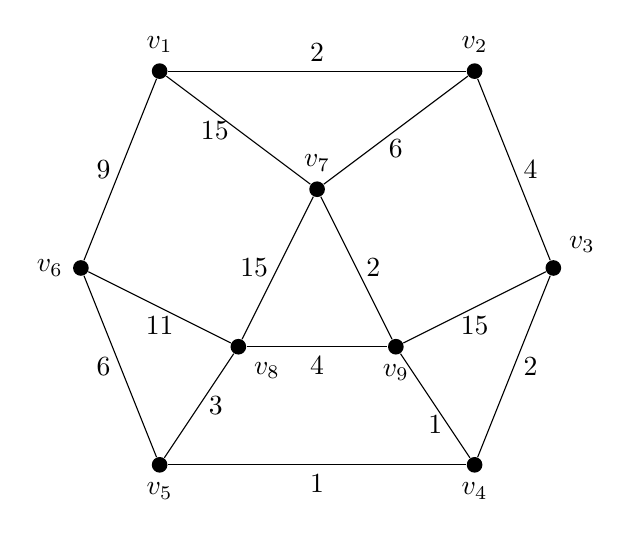
\begin{tikzpicture}
    \node[circle,fill,inner sep=2pt,label={north:$v_1$}] (v1) at (0,0) {};
    \node[circle,fill,inner sep=2pt,label={north:$v_2$}] (v2) at (4,0) {};
    \node[circle,fill,inner sep=2pt,label={north east:$v_3$}] (v3) at (5,-2.5) {};
    \node[circle,fill,inner sep=2pt,label={south:$v_4$}] (v4) at (4,-5) {};
    \node[circle,fill,inner sep=2pt,label={south:$v_5$}] (v5) at (0,-5) {};
    \node[circle,fill,inner sep=2pt,label={west:$v_6$}] (v6) at (-1,-2.5) {};
    
    \node[circle,fill,inner sep=2pt,label={north:$v_7$}] (v7) at (2,-1.5) {};
    \node[circle,fill,inner sep=2pt,label={south east:$v_8$}] (v8) at (1,-3.5) {};
    \node[circle,fill,inner sep=2pt,label={south:$v_9$}] (v9) at (3,-3.5) {};
    
    \path (v1) edge node[above] {$2$} (v2);
    \path (v2) edge node[right] {$4$} (v3);
    \path (v3) edge node[right] {$2$} (v4);
    \path (v4) edge node[below] {$1$} (v5);
    \path (v5) edge node[left] {$6$} (v6);
    \path (v6) edge node[left] {$9$} (v1);
    
    \path (v1) edge node[left] {$15$} (v7);
    \path (v2) edge node[below] {$6$} (v7);
    \path (v3) edge node[below] {$15$} (v9);
    \path (v4) edge node[below] {$1$} (v9);
    \path (v5) edge node[right] {$3$} (v8);
    \path (v6) edge node[below] {$11$} (v8);
    
    \path (v8) edge node[below] {$4$} (v9);
    \path (v7) edge node[left] {$15$} (v8);
    \path (v7) edge node[right] {$2$} (v9);
\end{tikzpicture}
\caption{Graph mit neun Knoten.}
\label{figure-dijkstra-aufgaben-g1}
\end{figure}

\item Bestimmen Sie im Graphen aus \autoref{figure-dijkstra-aufgaben-g1} den kürzesten Weg von $v_1$ nach $v_4$. Müssen Sie den Algorithmus erneut durchführen? Begründen Sie Ihre Antwort.
\item Bestimmen Sie im Graphen aus \autoref{figure-dijkstra-aufgaben-g1} den kürzesten Weg von $v_8$ nach $v_9$. Müssen Sie den Algorithmus erneut durchführen? Begründen Sie Ihre Antwort.
\item Bestimmen Sie die Lösung für die Eingangsfrage (\say{Welches ist der kürzeste Weg von Imstadt nach Oppenheim?}). Führen Sie dazu den Dijkstra-Algorithmus aus. \autoref{figure-dijkstra-aufgaben-g2} zeigt den Graphen.

\begin{figure}[htb]
\centering
\resizebox{!}{11cm}{
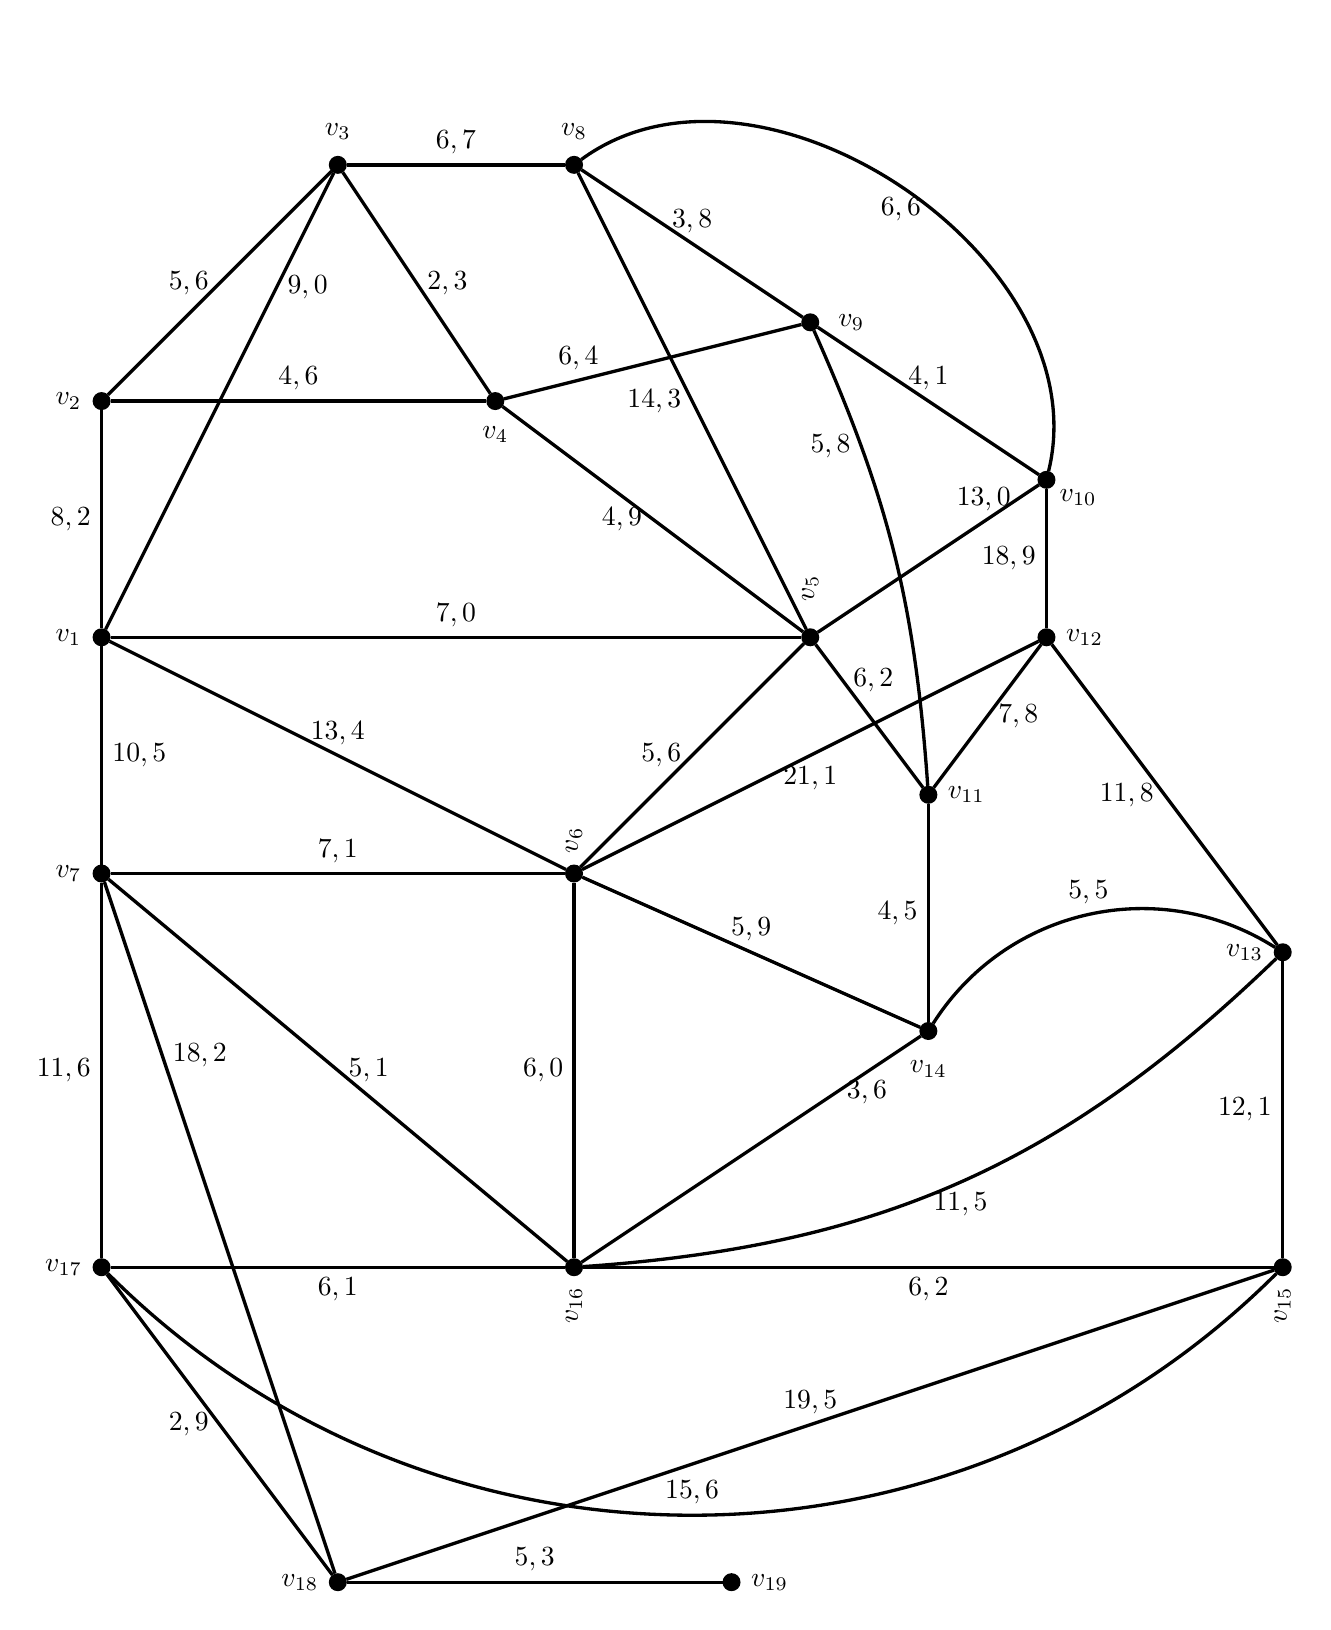
\begin{tikzpicture}
\begin{scope}[every node/.style={circle, thick, fill, draw, inner sep=0cm, minimum size=0.2cm}]
    \node[label={[label distance=0.1cm]180:$v_1$}] (v1) at (-3,0) {};
    \node[label={[label distance=0.1cm]180:$v_2$}] (v2) at (-3,3) {};
    \node[label={[label distance=0.1cm]90:$v_3$}] (v3) at (0,6) {};
    \node[label={[label distance=0.1cm]270:$v_4$}] (v4) at (2,3) {};
    \node[label={[label distance=0.3cm]90:\rotatebox{90}{$v_5$}}] (v5) at (6,0) {};
    \node[label={[label distance=0.1cm]90:\rotatebox{90}{$v_6$}}] (v6) at (3,-3) {};
    \node[label={[label distance=0.1cm]180:$v_7$}] (v7) at (-3,-3) {};
    \node[label={[label distance=0.1cm]90:$v_8$}] (v8) at (3,6) {};
    \node[label={[label distance=0.2cm]0:$v_9$}] (v9) at (6,4) {};
    \node[label={[label distance=0.1cm]350:$v_{10}$}] (v10) at (9,2) {};
    \node[label={[label distance=0.1cm]0:$v_{11}$}] (v11) at (7.5,-2) {};
    \node[label={[label distance=0.1cm]0:$v_{12}$}] (v12) at (9,0) {};
    \node[label={[label distance=0.1cm]180:$v_{13}$}] (v13) at (12,-4) {};
    \node[label={[label distance=0.1cm]270:$v_{14}$}] (v14) at (7.5,-5) {};
    \node[label={[label distance=0.1cm]270:\rotatebox{90}{$v_{15}$}}] (v15) at (12,-8) {};
    \node[label={[label distance=0.1cm]270:\rotatebox{90}{$v_{16}$}}] (v16) at (3,-8) {};
    \node[label={[label distance=0.1cm]180:$v_{17}$}] (v17) at (-3,-8) {};
    \node[label={[label distance=0.1cm]180:$v_{18}$}] (v18) at (0,-12) {};
    \node[label={[label distance=0.1cm]0:$v_{19}$}] (v19) at (5,-12) {};
\end{scope}
\begin{scope}[every edge/.style={draw=black, very thick}]
    \path (v1) edge node[left] {$8,2$} (v2);
    \path (v1) edge node[near end, right] {$9,0$} (v3);
    \path (v1) edge node[above] {$7,0$} (v5);
    \path (v1) edge node[above] {$13,4$} (v6);
    \path (v1) edge node[right] {$10,5$} (v7);
    \path (v2) edge node[left] {$5,6$} (v3);
    \path (v2) edge node[above] {$4,6$} (v4);
    \path (v3) edge node[right] {$2,3$} (v4);
    \path (v3) edge node[above] {$6,7$} (v8);
    \path (v4) edge node[left] {$4,9$} (v5);
    \path (v4) edge node[near start, above] {$6,4$} (v9);
    \path (v5) edge node[left] {$5,6$} (v6);
    \path (v5) edge node[left] {$14,3$} (v8);
    \path (v5) edge node[near end, above] {$13,0$} (v10);
    \path (v5) edge node[near start, right] {$6,2$} (v11);
    \path (v6) edge node[above] {$7,1$} (v7);
    \path (v6) edge node[above] {$5,9$} (v14);
    \path (v6) edge node[left] {$6,0$} (v16);
    \path (v7) edge node[right] {$5,1$} (v16);
    \path (v7) edge node[left] {$11,6$} (v17);
    \path (v7) edge node[right, near start] {$18,2$} (v18);
    \path (v8) edge node[above] {$3,8$} (v9);
    \path (v8) edge[bend left=70, below] node {$6,6$} (v10);
    \path (v9) edge node[above] {$4,1$} (v10);
    \path (v9) edge[bend left=10] node[near start, left] {$5,8$} (v11);
    \path (v10) edge node[left] {$18,9$} (v12);
    \path (v11) edge node[left] {$4,5$} (v14);
    \path (v12) edge node[right] {$7,8$} (v11);
    \path (v12) edge node[left] {$11,8$} (v13);
    \path (v12) edge node[below] {$21,1$} (v6);
    \path (v13) edge node[left] {$12,1$} (v15);
    \path (v13) edge[bend left=20, below] node {$11,5$} (v16);
    \path (v14) edge node[right, near start] {$3,6$} (v16);
    \path (v14) edge[bend left=45, above] node {$5,5$} (v13);
    \path (v15) edge node[below] {$6,2$} (v16);
    \path (v15) edge[bend left=45, above] node {$15,6$} (v17);
    \path (v15) edge node[above] {$19,5$} (v18);
    \path (v16) edge node[below] {$6,1$} (v17);
    \path (v17) edge node[left] {$2,9$} (v18);
    \path (v18) edge node[above] {$5,3$} (v19);
\end{scope}
\end{tikzpicture}
}
\caption{Graph mit $19$ Knoten.}
\label{figure-dijkstra-aufgaben-g2}
\end{figure}

\newpage

\begin{figure}[htb]
\centering
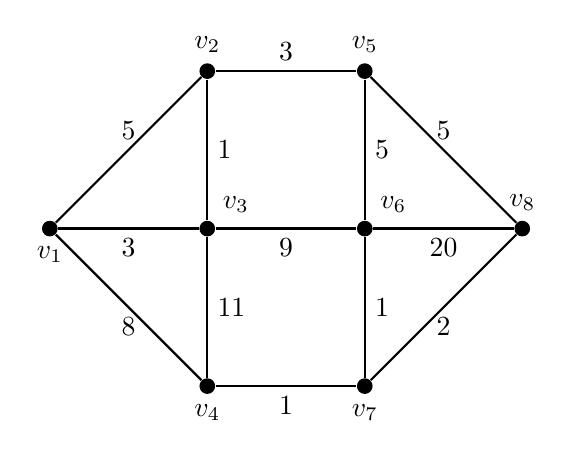
\begin{tikzpicture}
    \node[circle, fill, inner sep=2pt, label={[black]south:$v_1$}] (v1) at (0,0) {};
    \node[circle, fill, inner sep=2pt, label={[black]north:$v_2$}] (v2) at (2,2) {};
    \node[circle, fill, inner sep=2pt, label={[black]north east:$v_3$}] (v3) at (2,0) {};
    \node[circle, fill, inner sep=2pt, label={[black]south:$v_4$}] (v4) at (2,-2) {};
    
    \node[circle, fill, inner sep=2pt, label={north:$v_5$}] (v5) at (4,2) {};
    \node[circle, fill, inner sep=2pt, label={[black]north east:$v_6$}] (v6) at (4,0) {};
    \node[circle, fill, inner sep=2pt, label={south:$v_7$}] (v7) at (4,-2) {};
    
    \node[circle, fill, inner sep=2pt, label={north:$v_8$}] (v8) at (6,0) {};
    
    \path[thick] (v1) edge node[above] {$5$} (v2);
    \path[thick] (v1) edge node[below] {$3$} (v3);
    
    \path[thick] (v1) edge node[below] {$8$} (v4);
    
    \path[thick] (v2) edge node[above] {$3$} (v5);
    \path[thick] (v2) edge node[right] {$1$} (v3);
    \path[thick] (v3) edge node[below] {$9$} (v6);
    \path[thick] (v3) edge node[right] {$11$} (v4);
    \path[thick] (v4) edge node[below] {$1$} (v7);
    
    \path[thick] (v5) edge node[above] {$5$} (v8);
    \path[thick] (v5) edge node[right] {$5$} (v6);
    \path[thick] (v6) edge node[below] {$20$} (v8);
    \path[thick] (v6) edge node[right] {$1$} (v7);
    \path[thick] (v7) edge node[below] {$2$} (v8);
\end{tikzpicture}
\end{figure}

\end{enumerate}

\newpage

\begin{enumerate}
	\item Der Graph in \autoref{figure-graph-map-ch-solution} zeigt die Strassenkarte mit 17 Knoten.

\begin{figure}[htb]
\centering
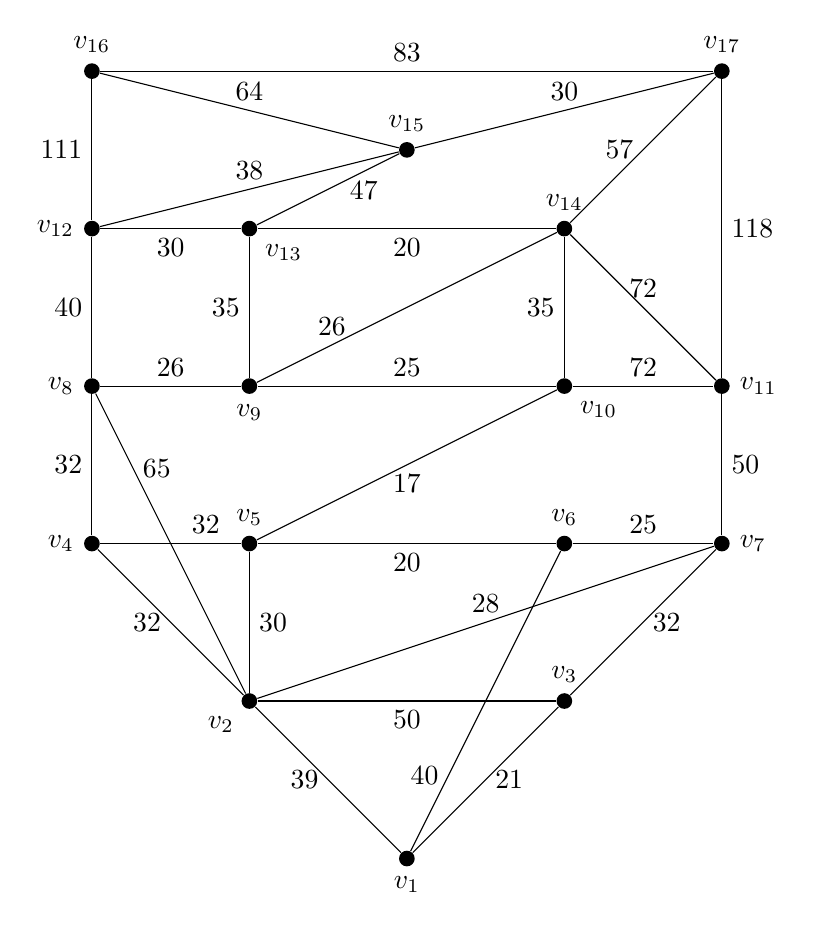
\begin{tikzpicture}
    \node[circle, fill, inner sep=2pt, label={south:$v_1$}] (v1) at (0,0) {};
    \node[circle, fill, inner sep=2pt, label={south west:$v_2$}] (v2) at (-2,2) {};
    \node[circle, fill, inner sep=2pt, label={$v_3$}] (v3) at (2,2) {};
    \node[circle, fill, inner sep=2pt, label={west:$v_4$}] (v4) at (-4,4) {};
    \node[circle, fill, inner sep=2pt, label={$v_5$}] (v5) at (-2,4) {};
    \node[circle, fill, inner sep=2pt, label={$v_6$}] (v6) at (2,4) {};
    \node[circle, fill, inner sep=2pt, label={east:$v_7$}] (v7) at (4,4) {};
    \node[circle, fill, inner sep=2pt, label={west:$v_8$}] (v8) at (-4,6) {};
    \node[circle, fill, inner sep=2pt, label={south:$v_9$}] (v9) at (-2,6) {};
    \node[circle, fill, inner sep=2pt, label={south east:$v_{10}$}] (v10) at (2,6) {};
    \node[circle, fill, inner sep=2pt, label={east:$v_{11}$}] (v11) at (4,6) {};
    \node[circle, fill, inner sep=2pt, label={west:$v_{12}$}] (v12) at (-4,8) {};
    \node[circle, fill, inner sep=2pt, label={south east:$v_{13}$}] (v13) at (-2,8) {};
    \node[circle, fill, inner sep=2pt, label={$v_{14}$}] (v14) at (2,8) {};
    \node[circle, fill, inner sep=2pt, label={$v_{15}$}] (v15) at (0,9) {};
    \node[circle, fill, inner sep=2pt, label={$v_{16}$}] (v16) at (-4,10) {};
    \node[circle, fill, inner sep=2pt, label={$v_{17}$}] (v17) at (4,10) {};
    \path (v1) edge node[left] {$39$} (v2);
    \path (v1) edge node[right] {$21$} (v3);
    \path (v1) edge node[left, near start] {$40$} (v6);
    \path (v2) edge node[below] {$50$} (v3);
    \path (v2) edge node[left] {$32$} (v4);
    \path (v2) edge node[right] {$30$} (v5);
    \path (v2) edge node[above] {$28$} (v7);
    \path (v2) edge node[right, near end] {$65$} (v8);
    \path (v3) edge node[right] {$32$} (v7);
    \path (v4) edge node[above, near end] {$32$} (v5);
    \path (v4) edge node[left] {$32$} (v8);
    \path (v5) edge node[below] {$20$} (v6);
    \path (v5) edge node[below] {$17$} (v10);
    \path (v6) edge node[above] {$25$} (v7);
    \path (v7) edge node[right] {$50$} (v11);
    \path (v8) edge node[above] {$26$} (v9);
    \path (v8) edge node[left] {$40$} (v12);
    \path (v9) edge node[above] {$25$} (v10);
    \path (v9) edge node[above, near start] {$26$} (v14);
    \path (v9) edge node[left] {$35$} (v13);
    \path (v10) edge node[left] {$35$} (v14);
    \path (v10) edge node[above] {$72$} (v11);
    \path (v11) edge node[above] {$72$} (v14);
    \path (v11) edge node[right] {$118$} (v17);
    \path (v12) edge node[below] {$30$} (v13);
    \path (v12) edge node[left] {$111$} (v16);
    \path (v12) edge node[above] {$38$} (v15);
    \path (v13) edge node[below, near end] {$47$} (v15);
    \path (v13) edge node[below] {$20$} (v14);
    \path (v14) edge node[left] {$57$} (v17);
    \path (v15) edge node[above] {$30$} (v17);
    \path (v15) edge node[above] {$64$} (v16);
    \path (v16) edge node[above] {$83$} (v17);
\end{tikzpicture}
\caption{Städte und Strassenkreuzungen werden zu Knoten.}
\label{figure-graph-map-ch-solution}
\end{figure}

\begin{multicols}{2}
\begin{itemize}
\item $v_1$ entspricht Olten
\item $v_2$ entspricht Solothurn
\item $v_3$ entspricht Dagmarsellen
\item $v_4$ entspricht Biel
\item $v_5$ entspricht einer Kreuzung
\item $v_6$ entspricht einer Kreuzung
\item $v_7$ entspricht einer Affoltern
\item $v_8$ entspricht Neuenburg
\item $v_9$ entspricht Kerzers
\item $v_{10}$ entspricht einer Kreuzung
\item $v_{11}$ entspricht Thun
\item $v_{12}$ entspricht Yverdon-les-Bains
\item $v_{13}$ entspricht einer Kreuzung
\item $v_{14}$ entspricht Freiburg
\item $v_{15}$ entspricht Lausanne
\item $v_{16}$ entspricht Genf
\item $v_{17}$ entspricht Montreux
\end{itemize}
\end{multicols}

\end{enumerate}

\newpage

\begin{enumerate}
	\item Wir führen den Dijkstra-Algorithmus für den Graphen aus \autoref{figure-dijkstra-aufgaben-g1} Schritt-für-Schritt aus und erhalten die Lösung aus \autoref{figure-dijkstra-aufgaben-g1-solution-1}.
	
\begin{figure}[htb]
\centering
\begin{minipage}{0.45\textwidth}
	\centering
	\begin{tikzpicture}
    \node[circle, fill, darkgreen, inner sep=2pt, label={[darkgreen]north:$v_1$}, label={[darkgreen]west:\textbf{0}}] (v1) at (0,0) {};
    \node[circle, fill, darkgreen, inner sep=2pt, label={[darkgreen]north:$v_2$}, label={[darkgreen]east:\textbf{2}}] (v2) at (4,0) {};
    \node[circle, fill, darkgreen, inner sep=2pt, label={[darkgreen]north east:$v_3$}, label={[darkgreen]east:\textbf{6}}] (v3) at (5,-2.5) {};
    \node[circle, fill, darkgreen, inner sep=2pt, label={[darkgreen]south:$v_4$}, label={[darkgreen]east:\textbf{8}}] (v4) at (4,-5) {};
    \node[circle, fill, darkgreen, inner sep=2pt, label={[darkgreen]south:$v_5$}, label={[darkgreen]west:\textbf{9}}] (v5) at (0,-5) {};
    \node[circle, fill, darkgreen, inner sep=2pt, label={[darkgreen]west:$v_6$}, label={[darkgreen]north east:\textbf{9}}] (v6) at (-1,-2.5) {};
    
    \node[circle, fill, darkgreen, inner sep=2pt, label={[darkgreen]north:$v_7$}, label={[darkgreen]east:\textbf{8}}] (v7) at (2,-1.5) {};
    \node[circle, fill, darkgreen, inner sep=2pt, label={[darkgreen]south east:$v_8$}, label={[darkgreen]north east:\textbf{12}}] (v8) at (1,-3.5) {};
    \node[circle, fill, darkgreen, inner sep=2pt, label={[darkgreen]south:$v_9$}, label={[darkgreen]north east:\textbf{9}}] (v9) at (3,-3.5) {};
    
    \path (v1) edge node[above] {$2$} node[darkgreen, below, thick] {$\leftarrow$}  (v2);
    \path (v2) edge node[right] {$4$} node[darkgreen, below, sloped, thick] {$\leftarrow$} (v3);
    \path (v3) edge node[right] {$2$} node[darkgreen, above, sloped, thick] {$\rightarrow$} (v4);
    \path (v4) edge node[below] {$1$} node[darkgreen, above, thick] {$\rightarrow$} (v5);
    \path (v5) edge node[left] {$6$} (v6);
    \path (v6) edge node[left] {$9$} node[darkgreen, below, thick, sloped] {$\rightarrow$} (v1);
    
    \path (v1) edge node[left] {$15$} (v7);
    \path (v2) edge node[below] {$6$} node[darkgreen, above, thick, sloped] {$\rightarrow$} (v7);
    \path (v3) edge node[below] {$15$} (v9);
    \path (v4) edge node[below] {$1$} node[darkgreen, above, thick, sloped] {$\rightarrow$} (v9);
    \path (v5) edge node[right] {$3$} node[darkgreen, above, thick, sloped] {$\leftarrow$} (v8);
    \path (v6) edge node[below] {$11$} (v8);
    
    \path (v8) edge node[below] {$4$} (v9);
    \path (v7) edge node[left] {$15$} (v8);
    \path (v7) edge node[right] {$2$} (v9);
    
    \begin{pgfonlayer}{background}
        \draw[rounded corners=2em, line width=2.25em, yellow!30, cap=round] (v1.center) -- (v2.center) -- (v3.center) -- (v4.center) -- (v9.center);
    \end{pgfonlayer}
\end{tikzpicture}
\caption{Der kürzeste Weg von $v_1$ zu $v_9$ lautet $p =(v_1, v_2, v_3, v_4, v_9)$.}
\label{figure-dijkstra-aufgaben-g1-solution-1}
\end{minipage}
\hfill
\begin{minipage}{0.45\textwidth}
	\centering
	\begin{tikzpicture}
    \node[circle, fill, darkgreen, inner sep=2pt, label={[darkgreen]north:$v_1$}, label={[darkgreen]west:\textbf{2}}] (v1) at (0,0) {};
    \node[circle, fill, darkgreen, inner sep=2pt, label={[darkgreen]north:$v_2$}, label={[darkgreen]east:\textbf{0}}] (v2) at (4,0) {};
    \node[circle, fill, darkgreen, inner sep=2pt, label={[darkgreen]north east:$v_3$}, label={[darkgreen]east:\textbf{4}}] (v3) at (5,-2.5) {};
    \node[circle, fill, darkgreen, inner sep=2pt, label={[darkgreen]south:$v_4$}, label={[darkgreen]east:\textbf{6}}] (v4) at (4,-5) {};
    \node[circle, fill, darkgreen, inner sep=2pt, label={[darkgreen]south:$v_5$}, label={[darkgreen]west:\textbf{7}}] (v5) at (0,-5) {};
    \node[circle, fill, darkgreen, inner sep=2pt, label={[darkgreen]west:$v_6$}, label={[darkgreen]north east:\textbf{11}}] (v6) at (-1,-2.5) {};
    
    \node[circle, fill, darkgreen, inner sep=2pt, label={[darkgreen]north:$v_7$}, label={[darkgreen]east:\textbf{6}}] (v7) at (2,-1.5) {};
    \node[circle, fill, darkgreen, inner sep=2pt, label={[darkgreen]south east:$v_8$}, label={[darkgreen]north east:\textbf{10}}] (v8) at (1,-3.5) {};
    \node[circle, fill, darkgreen, inner sep=2pt, label={[darkgreen]south:$v_9$}, label={[darkgreen]north east:\textbf{7}}] (v9) at (3,-3.5) {};
    
    \path (v1) edge node[above] {$2$} node[darkgreen, below, thick] {$\rightarrow$}  (v2);
    \path (v2) edge node[right] {$4$} node[darkgreen, below, thick, sloped] {$\leftarrow$} (v3);
    \path (v3) edge node[right] {$2$} node[darkgreen, above, thick, sloped] {$\rightarrow$} (v4);
    \path (v4) edge node[below] {$1$} node[darkgreen, above, thick] {$\rightarrow$} (v5);
    \path (v5) edge node[left] {$6$} (v6);
    \path (v6) edge node[left] {$9$} node[darkgreen, below, thick, sloped] {$\rightarrow$} (v1);
    
    \path (v1) edge node[left] {$15$} (v7);
    \path (v2) edge node[below] {$6$} node[darkgreen, above, thick, sloped] {$\rightarrow$} (v7);
    \path (v3) edge node[below] {$15$} (v9);
    \path (v4) edge node[below] {$1$} node[darkgreen, above, thick, sloped] {$\rightarrow$} (v9);
    \path (v5) edge node[right] {$3$} node[darkgreen, above, thick, sloped] {$\leftarrow$} (v8);
    \path (v6) edge node[below] {$11$} (v8);
    
    \path (v8) edge node[below] {$4$} (v9);
    \path (v7) edge node[left] {$15$} (v8);
    \path (v7) edge node[right] {$2$} (v9);
    
    \begin{pgfonlayer}{background}
        \draw[rounded corners=2em, line width=2.25em, yellow!30, cap=round] (v2.center) -- (v3.center) -- (v4.center) -- (v5.center);
    \end{pgfonlayer}
	\end{tikzpicture}
	\caption{Der kürzeste Weg von $v_2$ zu $v_5$ lautet $p = (v_2, v_3, v_4, v_5).$}
	\label{figure-dijkstra-aufgaben-g1-solution-2}
\end{minipage}
\end{figure}

	\item Der Algorithmus von Dijkstra liefert für einen Startknoten die kürzesten Wege zu allen anderen Knoten. Da der Startknoten gleich bleibt, können wir das Ergebnis aus der ersten Teilaufgabe wiederverwenden. Der kürzeste Weg lautet somit $p = (v_1, v_2, v_3,v _4)$.

	\item Da der Startknoten sich verändert hat, müssen wir den Dijkstra-Algorithmus erneut durchführen. Wir führen deshalb den Algorithmus für den Graphen aus \autoref{figure-dijkstra-aufgaben-g1} Schritt-für-Schritt aus und erhalten die Lösung aus \autoref{figure-dijkstra-aufgaben-g1-solution-2}.

\item Wir müssen den kürzesten Weg von $v_1$ nach $v_18$ bestimmen. Wir führen deshalb den Algorithmus für den Graphen aus \autoref{figure-dijkstra-aufgaben-g1} Schritt-für-Schritt aus und erhalten die Lösung aus \autoref{figure-dijkstra-aufgaben-g2-solution}.

\begin{figure}[htb]
\centering
\resizebox{!}{19cm}{
\begin{tikzpicture}
\begin{scope}[every node/.style={circle, thick, fill, darkgreen, draw, inner sep=0cm, minimum size=0.2cm}]
    \node[label={[label distance=0.1cm]180:$v_1$}, label={[darkgreen]north west:\textbf{0}}] (v1) at (-3,0) {};
    \node[label={[label distance=0.1cm]180:$v_2$}, label={[darkgreen]north:\textbf{8,2}}] (v2) at (-3,3) {};
    \node[label={[label distance=0.1cm]90:$v_3$}, label={[darkgreen]west:\textbf{9}}] (v3) at (0,6) {};
    \node[label={[label distance=0.1cm]270:$v_4$}, label={[darkgreen]north east:\textbf{11,3}}] (v4) at (2,3) {};
    \node[label={[label distance=0.3cm]90:\rotatebox{90}{$v_5$}}, label={[darkgreen]east:\textbf{7}}] (v5) at (6,0) {};
    \node[label={[label distance=0.1cm]90:\rotatebox{90}{$v_6$}}, label={[darkgreen]south west:\textbf{12,6}}] (v6) at (3,-3) {};
    \node[label={[label distance=0.1cm]180:$v_7$}, label={[darkgreen]north west:\textbf{10,5}}] (v7) at (-3,-3) {};
    \node[label={[label distance=0.1cm]90:$v_8$}, label={[darkgreen]south west:\textbf{15,7}}] (v8) at (3,6) {};
    \node[label={[label distance=0.2cm]0:$v_9$}, label={[darkgreen]north:\textbf{17,4}}] (v9) at (6,4) {};
    \node[label={[label distance=0.1cm]350:$v_{10}$}, label={[darkgreen]north east:\textbf{20}}] (v10) at (9,2) {};
    \node[label={[label distance=0.1cm]0:$v_{11}$}, label={[darkgreen]west:\textbf{13,2}}] (v11) at (7.5,-2) {};
    \node[label={[label distance=0.1cm]0:$v_{12}$}, label={[darkgreen]north west:\textbf{21}}] (v12) at (9,0) {};
    \node[label={[label distance=0.1cm]180:$v_{13}$}, label={[darkgreen]east:\textbf{23,2}}] (v13) at (12,-4) {};
    \node[label={[label distance=0.1cm]270:$v_{14}$}, label={[darkgreen]east:\textbf{17,7}}] (v14) at (7.5,-5) {};
    \node[label={[label distance=0.1cm]270:\rotatebox{90}{$v_{15}$}}, label={[darkgreen]east:\textbf{21,8}}] (v15) at (12,-8) {};
    \node[label={[label distance=0.5cm]270:\rotatebox{90}{$v_{16}$}}, label={[darkgreen]south east:\textbf{15,6}}] (v16) at (3,-8) {};
    \node[label={[label distance=0.1cm]180:$v_{17}$}, label={[darkgreen]north east:\textbf{21,7}}] (v17) at (-3,-8) {};
    \node[label={[label distance=0.1cm]180:$v_{18}$}, label={[darkgreen]north east:\textbf{24,6}}] (v18) at (0,-12) {};
    \node[label={[label distance=0.1cm]0:$v_{19}$}, label={[darkgreen]north:\textbf{30,1}}] (v19) at (5,-12) {};
\end{scope}
\begin{scope}[every edge/.style={draw=black, thick}]
    \path (v1) edge node[left] {$8,2$} node[darkgreen, below, near end, sloped] {$\leftarrow$} (v2);
    \path (v1) edge node[near end, right] {$9,0$} node[darkgreen, above, sloped, near end] {$\leftarrow$} (v3);
    \path (v1) edge node[above] {$7,0$} node[darkgreen, below, near end] {$\leftarrow$} (v5);
    \path (v1) edge node[right] {$10,5$} node[darkgreen, above, sloped, near end] {$\leftarrow$} (v7);
    
    \path (v3) edge node[right] {$2,3$} node[darkgreen, below, sloped, near end] {$\leftarrow$} (v4);
    \path (v3) edge node[above] {$6,7$} node[darkgreen, above, near end] {$\leftarrow$} (v8);
    
    \path (v4) edge node[near start, above] {$6,4$} node[darkgreen, below, sloped, near end] {$\leftarrow$} (v9);
    
    \path (v5) edge node[left] {$5,6$} node[darkgreen, below, near start, sloped] {$\leftarrow$} (v6);
    \path (v5) edge node[near end, above] {$13,0$} node[darkgreen, below, near end, sloped] {$\leftarrow$} (v10);
    \path (v5) edge node[near start, right] {$6,2$} node[darkgreen, below, near end, sloped] {$\leftarrow$} (v11);
    
    \path (v7) edge node[right] {$5,1$} node[darkgreen, below, sloped, near end] {$\leftarrow$} (v16);
    \path (v11) edge node[left] {$4,5$} node[darkgreen, above, sloped, near end] {$\leftarrow$}  (v14);
    \path (v12) edge node[right] {$7,8$} node[darkgreen, below, sloped, near start] {$\leftarrow$} (v11);
    \path (v14) edge[bend left=45, above] node {$5,5$} node[darkgreen, below, sloped, near end] {$\leftarrow$} (v13);
    \path (v15) edge node[below] {$6,2$} node[darkgreen, above, near start] {$\leftarrow$} (v16);
    \path (v16) edge node[below] {$6,1$} node[darkgreen, above, near end] {$\rightarrow$} (v17);
    \path (v17) edge node[left] {$2,9$} node[darkgreen, above, sloped, near end] {$\leftarrow$} (v18);
    \path (v18) edge node[above] {$5,3$} node[darkgreen, below, near end] {$\leftarrow$} (v19);
    
    \path (v1) edge node[above] {$13,4$} (v6);
    \path (v2) edge node[left] {$5,6$} (v3);
    \path (v2) edge node[above] {$4,6$} (v4);
    \path (v4) edge node[left] {$4,9$} (v5);
    \path (v5) edge node[left] {$14,3$} (v8);
    \path (v6) edge node[above] {$7,1$} (v7);
    \path (v6) edge node[above] {$5,9$} (v14);
    \path (v6) edge node[left] {$6,0$} (v16);
    \path (v7) edge node[left] {$11,6$} (v17);
    \path (v7) edge node[right, near start] {$18,2$} (v18);
    \path (v8) edge node[above] {$3,8$} (v9);
    \path (v8) edge[bend left=70, below] node {$6,6$} (v10);
    \path (v9) edge node[above] {$4,1$} (v10);
    \path (v9) edge[bend left=10] node[near start, left] {$5,8$} (v11);
    \path (v10) edge node[right] {$18,9$} (v12);
    \path (v12) edge node[left] {$11,8$} (v13);
    \path (v12) edge node[below] {$21,1$} (v6);
    \path (v13) edge node[left] {$12,1$} (v15);
    \path (v13) edge[bend left=20, below] node {$11,5$} (v16);
    \path (v14) edge node[right, near start] {$3,6$} (v16);
    \path (v15) edge[bend left=45, above] node {$15,6$} (v17);
    \path (v15) edge node[above] {$19,5$} (v18);
\end{scope}
\end{tikzpicture}
}
\caption{Der kürzeste Weg von $v_1$ zu $v_{18}$ lautet $p = (v_1, v_7, v_{16}, v_{17}, v_{18})$.}
\label{figure-dijkstra-aufgaben-g2-solution}
\end{figure}


\end{enumerate}